\documentclass[10pt,a4paper,twocolumn]{article}

\usepackage[utf8]{inputenc}
\usepackage[T1]{fontenc}
\usepackage[english]{babel}
\usepackage[top=2.2cm, bottom=2.5cm, left=1.9cm, right=1.9cm, columnsep=0.8cm]{geometry}
\usepackage{amsmath, amssymb}
\usepackage{graphicx}
\usepackage{siunitx}
\usepackage{microtype}
\usepackage[font=small, labelfont=bf]{caption}
\usepackage[backend=biber, style=numeric-comp, sorting=none, maxbibnames=3, giveninits=true, doi=true]{biblatex}
\addbibresource{references.bib}
\usepackage{xcolor}
\definecolor{linkblue}{RGB}{25, 55, 125}
\usepackage[colorlinks=true, linkcolor=linkblue, citecolor=linkblue, urlcolor=linkblue]{hyperref}

\setlength{\parindent}{1em}
\setlength{\parskip}{0pt}

\title{\textbf{A Stochastic Metric-Topological Neighbor Rule\\for the Vicsek Model}}
\author{Rene-Marcel Lehner\\[2pt]
\small Department of Physics, TU Dortmund University}
\date{\small Condensed manuscript of the bachelor thesis
``Analyse und Simulation neuronaler Schwarmdynamik''\\
\small (TU Dortmund University, Kierfeld group, 2023). Prepared in 2026.}

\begin{document}

\twocolumn[
\maketitle
\begin{center}
\begin{minipage}{0.86\textwidth}
\small
\textbf{Abstract.}
Collective motion models describe how simple local rules produce
coherent swarms. A central modeling choice is how each agent selects
its neighbors: metric models use all agents within a fixed radius,
topological models use a fixed number of nearest neighbors. Purely
topological selection destabilizes the classic Vicsek model and
produces fragmented micro-flocks. This thesis introduced a stochastic
metric-topological rule: each agent draws $k$ neighbors uniformly at
random from all agents within its metric radius, resampled at every
time step. The sampled average is an unbiased Monte Carlo estimate of
the full Vicsek interaction, with $k$ acting as the sample size. In
simulations with up to $N=2000$ agents, the rule removes the
fragmentation of the topological model and reproduces Vicsek behavior
under the evaluated observables. The mean squared deviation of the
order parameter falls rapidly with $k$; for $k=6$ the two models are
nearly indistinguishable. A second part of the thesis explored
multi-agent reinforcement learning (MARL) as a way to replace
hand-written interaction rules with learned ones. An actor-critic
pipeline around the C++ simulation was implemented and ran end to end,
but training did not produce an interpretable policy. That part is
reported as a documented negative result.
\end{minipage}
\end{center}
\vspace{1.2em}
]

\section{Introduction}

Swarms of starlings, schools of fish, and herds of animals show a
remarkable property: complex collective behavior emerges from simple
individual decisions. Collective motion is studied across physics,
biology, computer science, and robotics
\cite{vicsek1995, CollectiveMotionVicsek2012, AerialSwarmRobotics,
RoboticSwarmInformation2019}. The foundational mathematical
description is the Vicsek model \cite{vicsek1995}: point-like agents
move at constant speed and align their heading with the average
heading of their neighbors, disturbed by noise. Many later models,
including the Boids model \cite{reynolds1987}, build on this idea.

A key modeling decision is hidden in the word ``neighbors''.
\emph{Metric} models let an agent interact with everyone inside a
fixed radius $r$. \emph{Topological} models let it interact with a
fixed number $k$ of nearest agents, regardless of distance.
Observations of real bird flocks support topological interactions
\cite{InteractionRulingAnimal2007}, and topological models show
richer phase behavior \cite{TopologicalFlockingModels2021}. However,
in the regimes studied in this thesis, purely topological selection
destabilizes the Vicsek dynamics: the swarm fragments into many small,
short-ranged packets instead of forming large coherent structures.

This manuscript summarizes the two contributions of the underlying
bachelor thesis:

\begin{enumerate}
    \setlength\itemsep{0pt}
    \item A \textbf{stochastic metric-topological neighbor rule},
    introduced in this thesis, that keeps the fixed neighbor count of
    topological models while recovering the stability of the metric
    Vicsek model. Its agreement with the Vicsek model is evaluated
    quantitatively.
    \item An exploratory \textbf{multi-agent reinforcement learning
    (MARL) extension} in which agents were meant to learn alignment
    behavior from a global objective instead of a fixed local rule.
    The pipeline was implemented and ran, but training was not
    successful. It is included as an honest negative result.
\end{enumerate}

\section{Background: the Vicsek model}

\begin{figure}[tb]
    \centering
    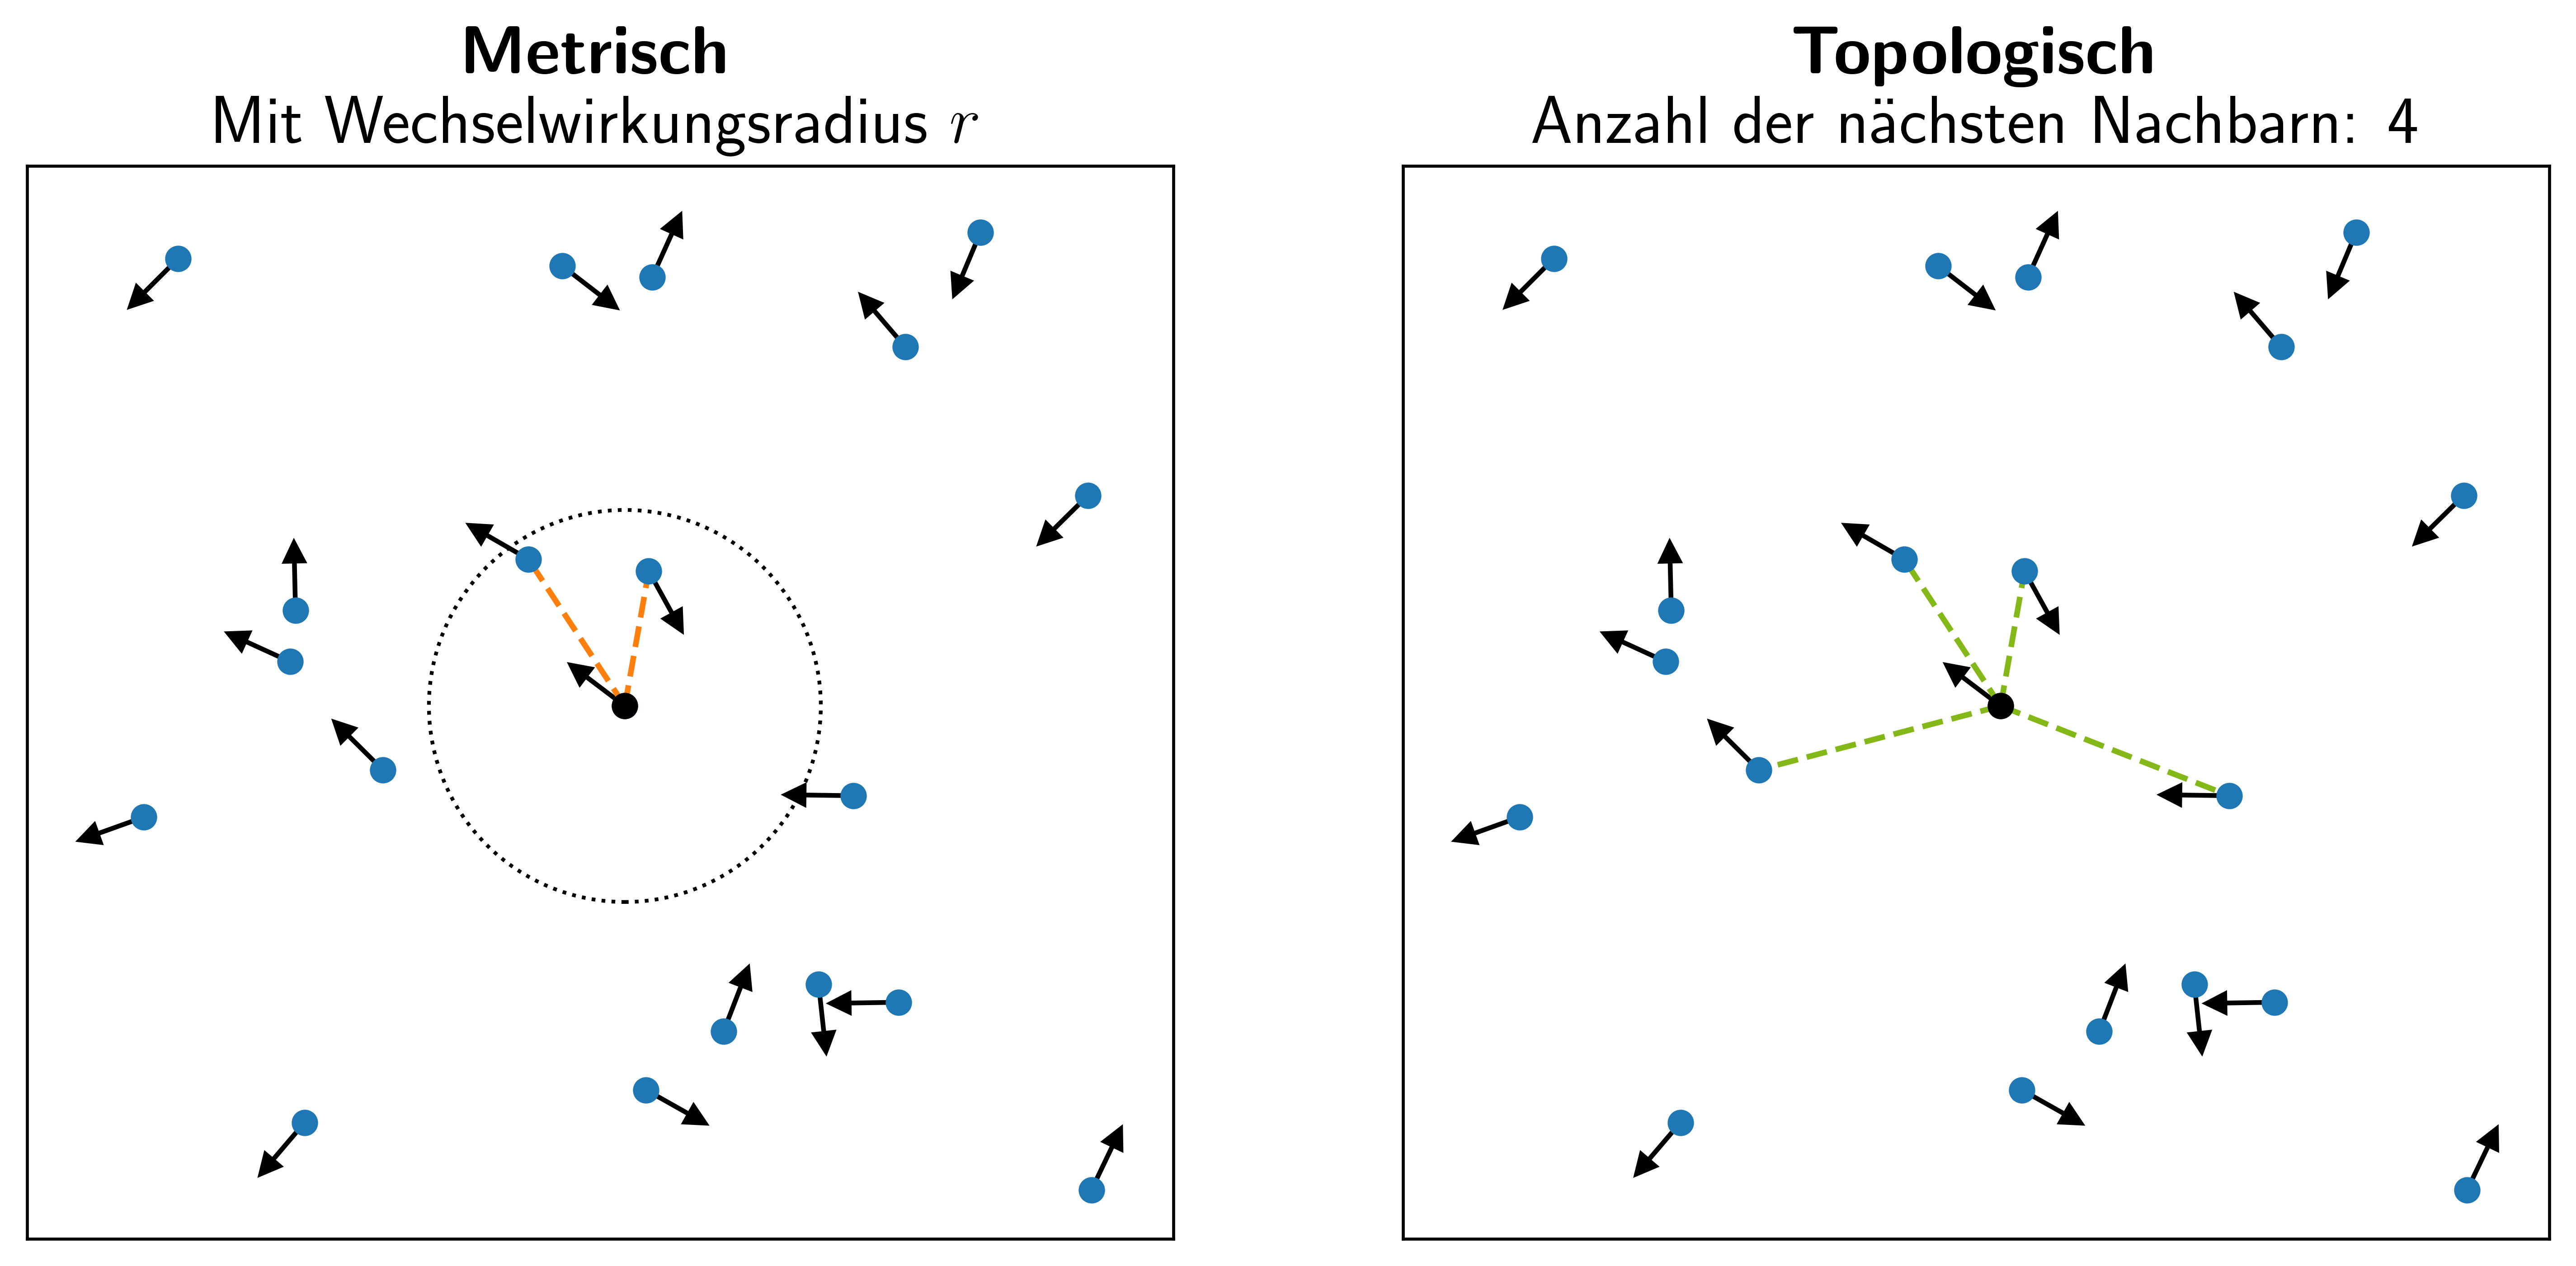
\includegraphics[width=\linewidth]{figures/metric_vs_topologic.png}
    \caption{Metric versus topological neighbor selection. Left: a
    metric agent (black) interacts with all agents inside its radius
    $r$ (dotted circle, orange links). Right: a topological agent
    interacts with its $k=4$ nearest agents (green links), however far
    away they are. Figure from the thesis; panel titles are in German
    (``Metrisch'' means metric, ``Topologisch'' means topological).}
    \label{fig:concept}
\end{figure}

The Vicsek model \cite{vicsek1995} describes $N$ agents in a square
box of side length $L$ with periodic boundaries. All agents move at
the same constant speed $v_0$. The only degree of freedom of agent
$i$ is its heading $\theta_i$. Positions advance with a simple Euler
step,
\begin{equation}
    \tilde{\vec{x}}_i(\tilde{t}+1)
    = \tilde{\vec{x}}_i(\tilde{t})
    + \tilde{\vec{v}}_i(\tilde{t}) \, \Delta\tilde{t},
    \label{eq:euler}
\end{equation}
where all quantities are made dimensionless with the interaction
radius $r$ and the speed $v_0$. The new heading is the average heading
of all neighbors within the radius $r$ (including the agent itself)
plus a noise term,
\begin{equation}
    \theta_i(\tilde{t}+1)
    = \langle\theta(\tilde{t})\rangle_r + \Delta\theta,
    \qquad
    \Delta\theta \sim \mathcal{U}\!\left[-\tfrac{\eta}{2},
    \tfrac{\eta}{2}\right],
    \label{eq:update}
\end{equation}
with the circular average
\begin{equation}
    \langle\theta(\tilde{t})\rangle_r
    = \arctan\!\left[
    \frac{\langle\sin\theta(\tilde{t})\rangle_r}
         {\langle\cos\theta(\tilde{t})\rangle_r}\right].
    \label{eq:rule}
\end{equation}
The noise strength $\eta$ controls the macroscopic state. The degree
of global alignment is measured by the order parameter
\begin{equation}
    v_a = \frac{1}{N v_0}\left|\sum_{i=1}^{N}\vec{v}_i\right|
    \in [0, 1],
    \label{eq:orderparam}
\end{equation}
which is $1$ for a perfectly aligned swarm and close to $0$ for a
disordered one. Following the original work, all simulations use
$v_0 = \num{0.03}$ (in units of $r$ per step) and are evaluated
through $v_a$ as a function of $\eta$, $N$, and the density
$\rho = N/L^2$.

Figure~\ref{fig:concept} illustrates the two established neighbor
definitions. The topological variant replaces the radius criterion in
Eq.~\eqref{eq:rule} with the $k$ nearest agents.

\subsection{Why purely topological selection fails here}

\begin{figure*}[tb]
    \centering
    \begin{tabular}{ccc}
    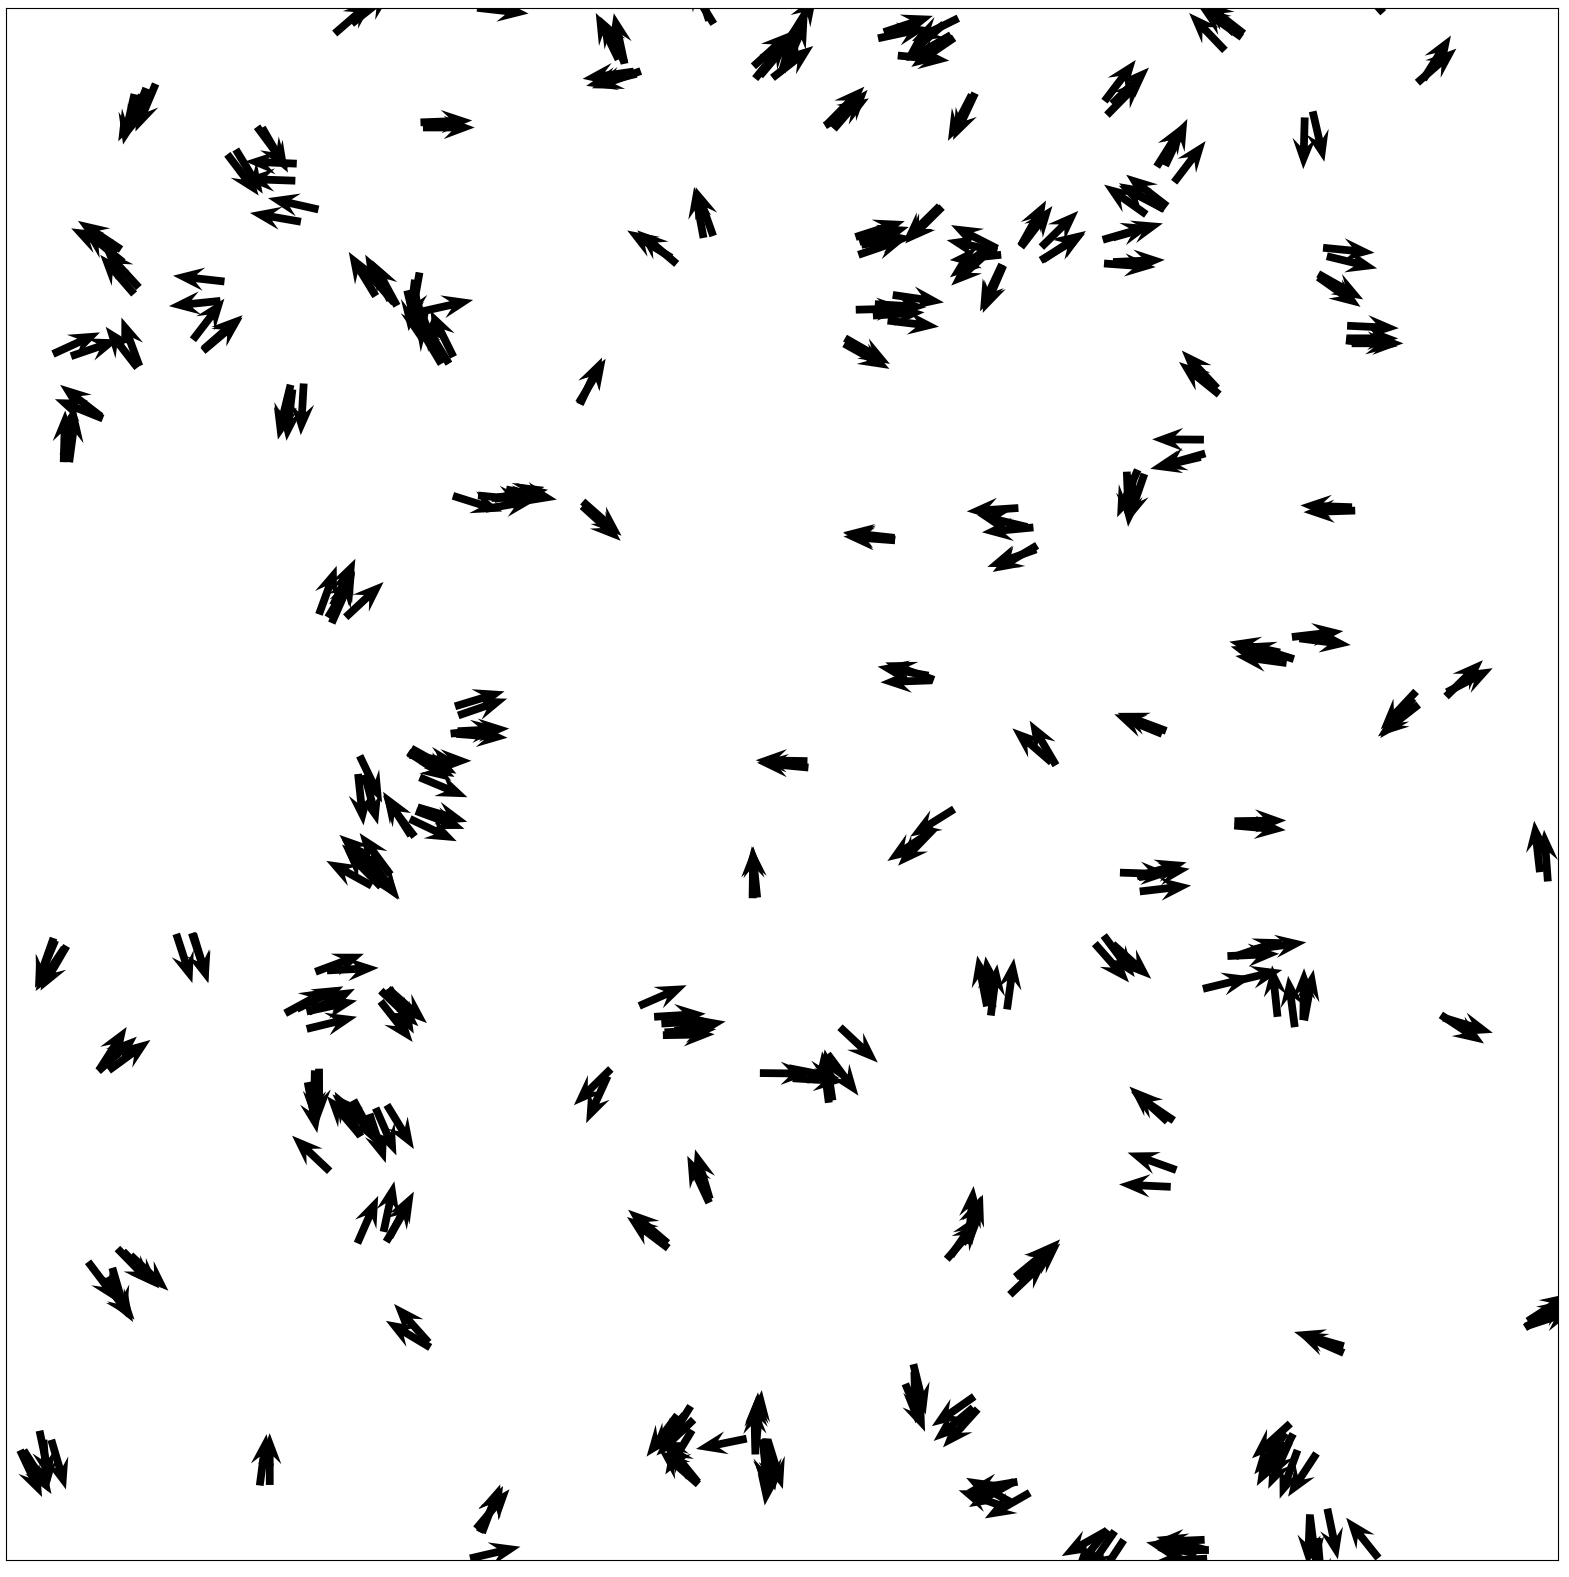
\includegraphics[width=0.28\textwidth]{figures/Snapshot_k1_n0.4.png} &
    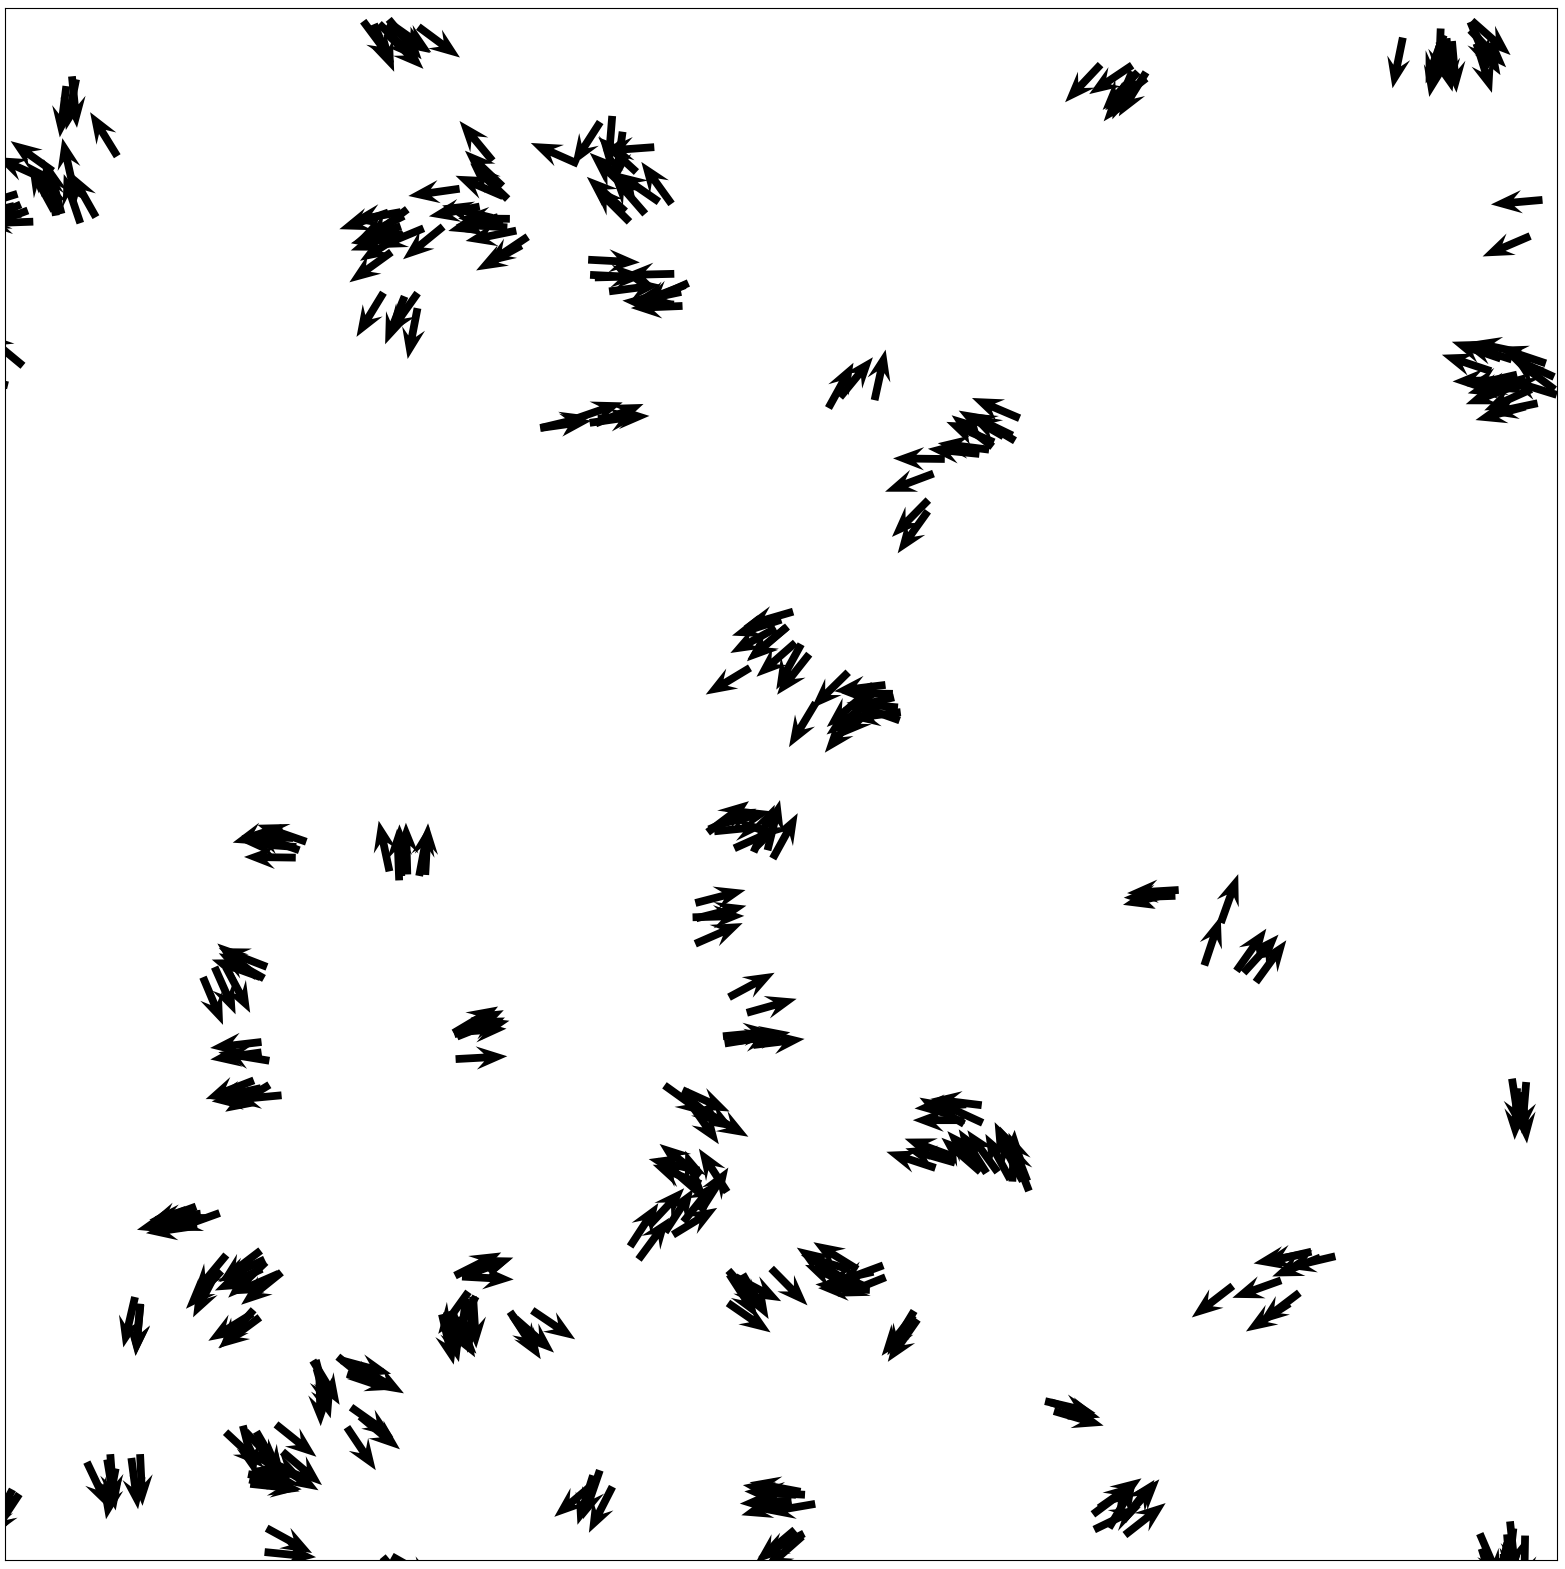
\includegraphics[width=0.28\textwidth]{figures/Snapshot_k2_n0.6.png} &
    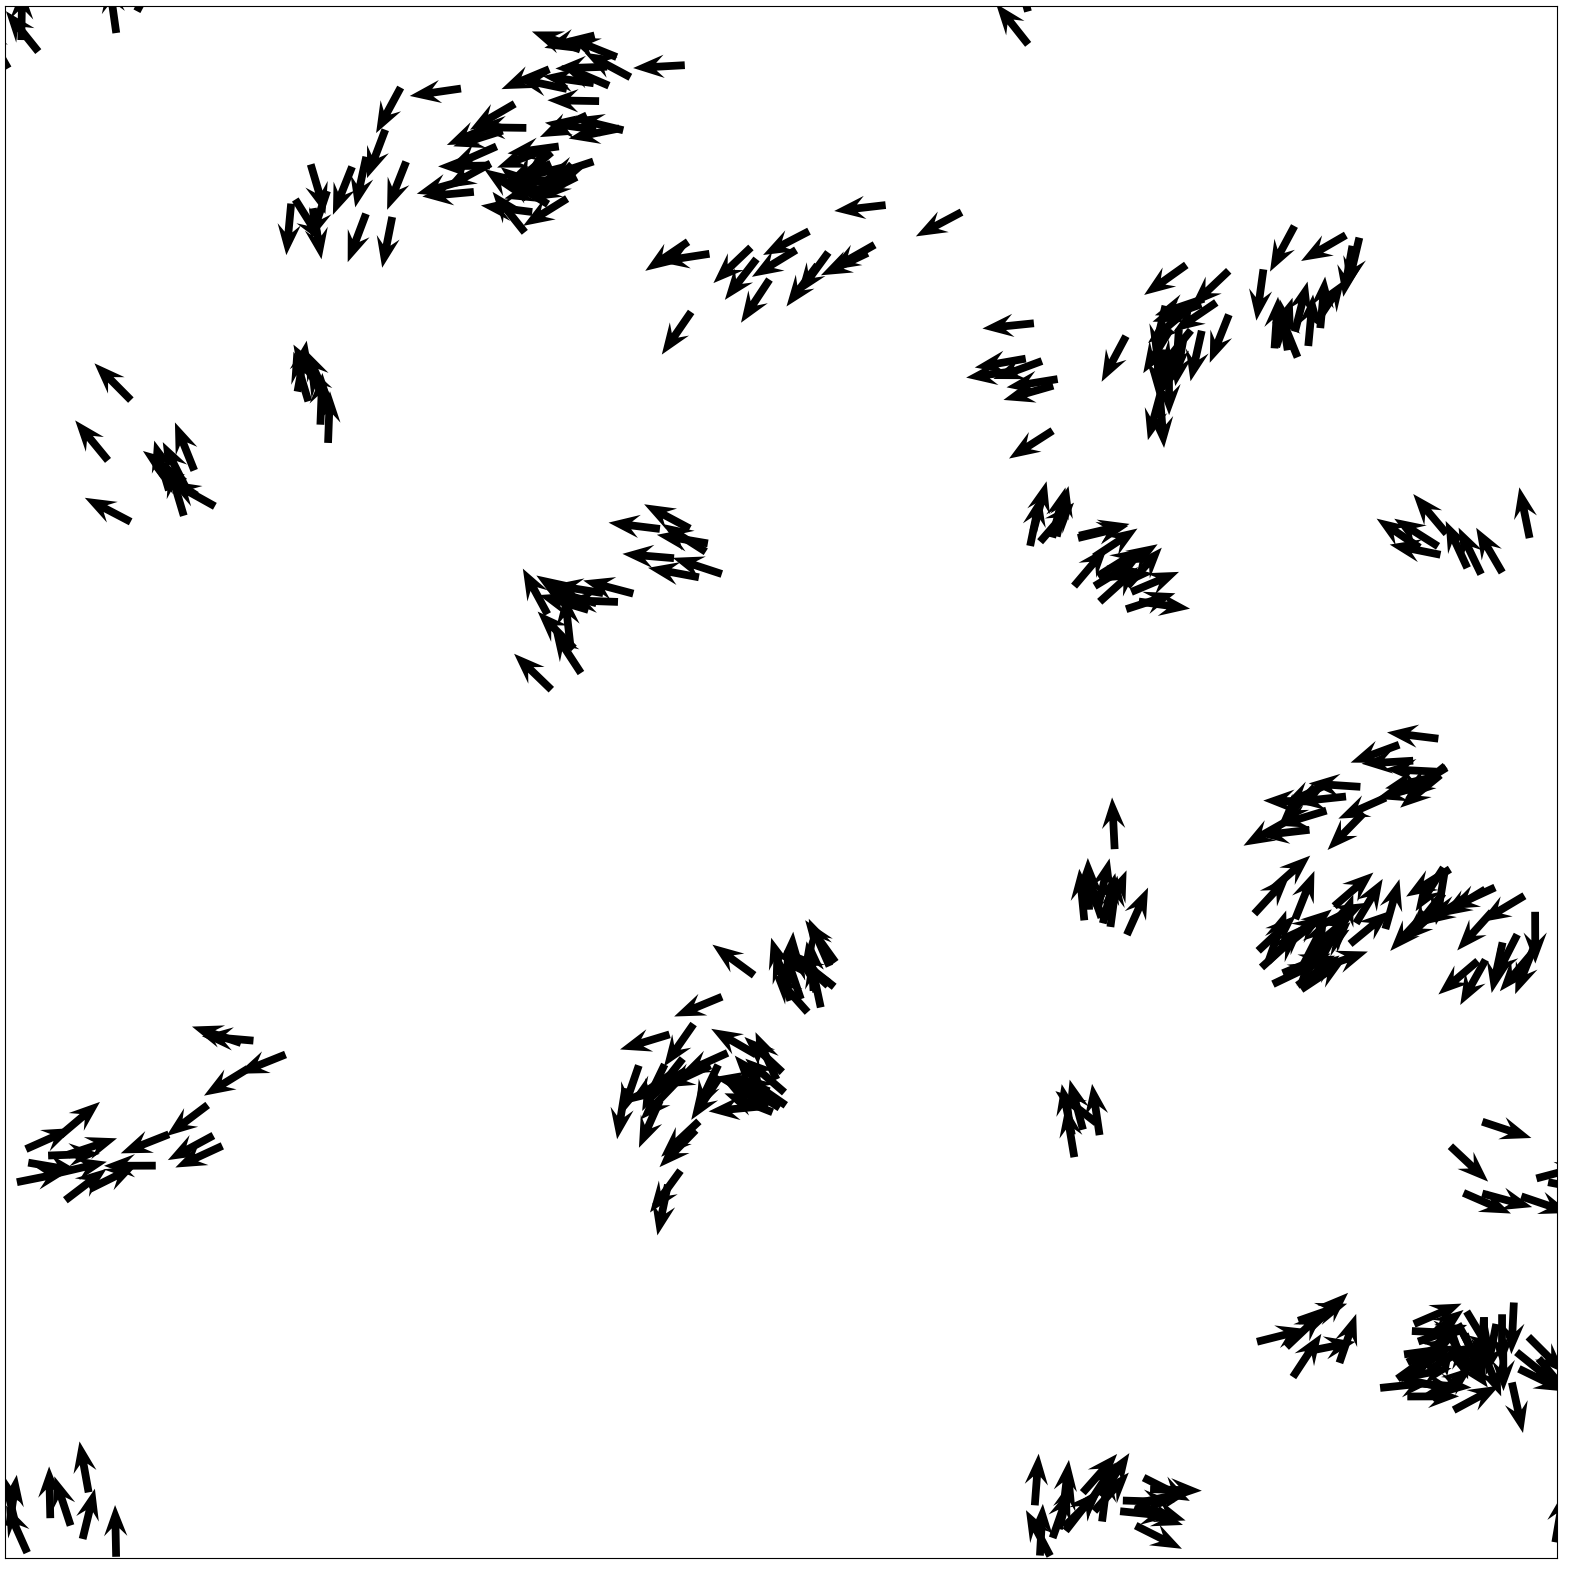
\includegraphics[width=0.28\textwidth]{figures/Snapshot_k4_n1.0.png} \\
    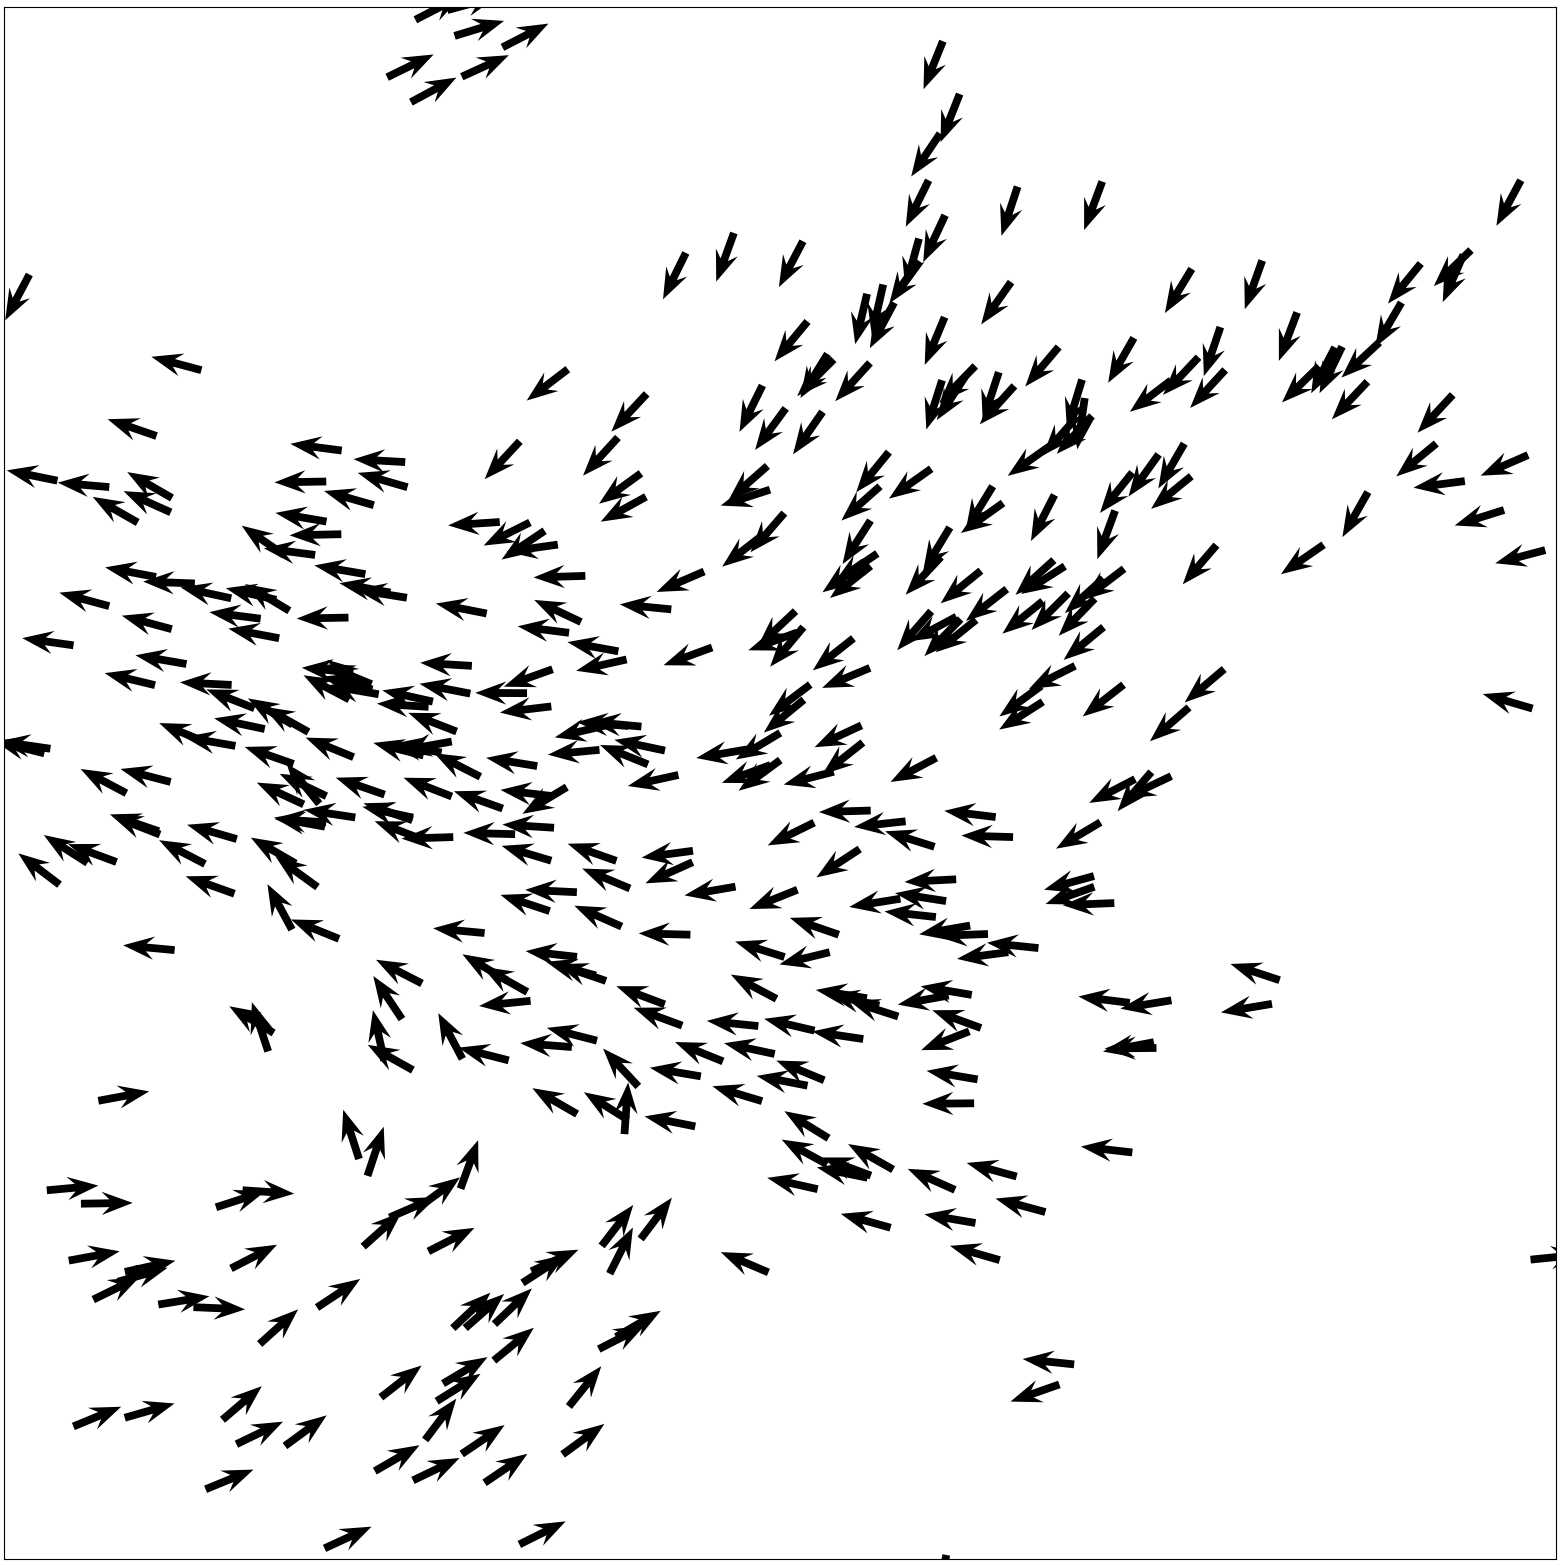
\includegraphics[width=0.28\textwidth]{figures/Snapshot_rk1_n0.4.png} &
    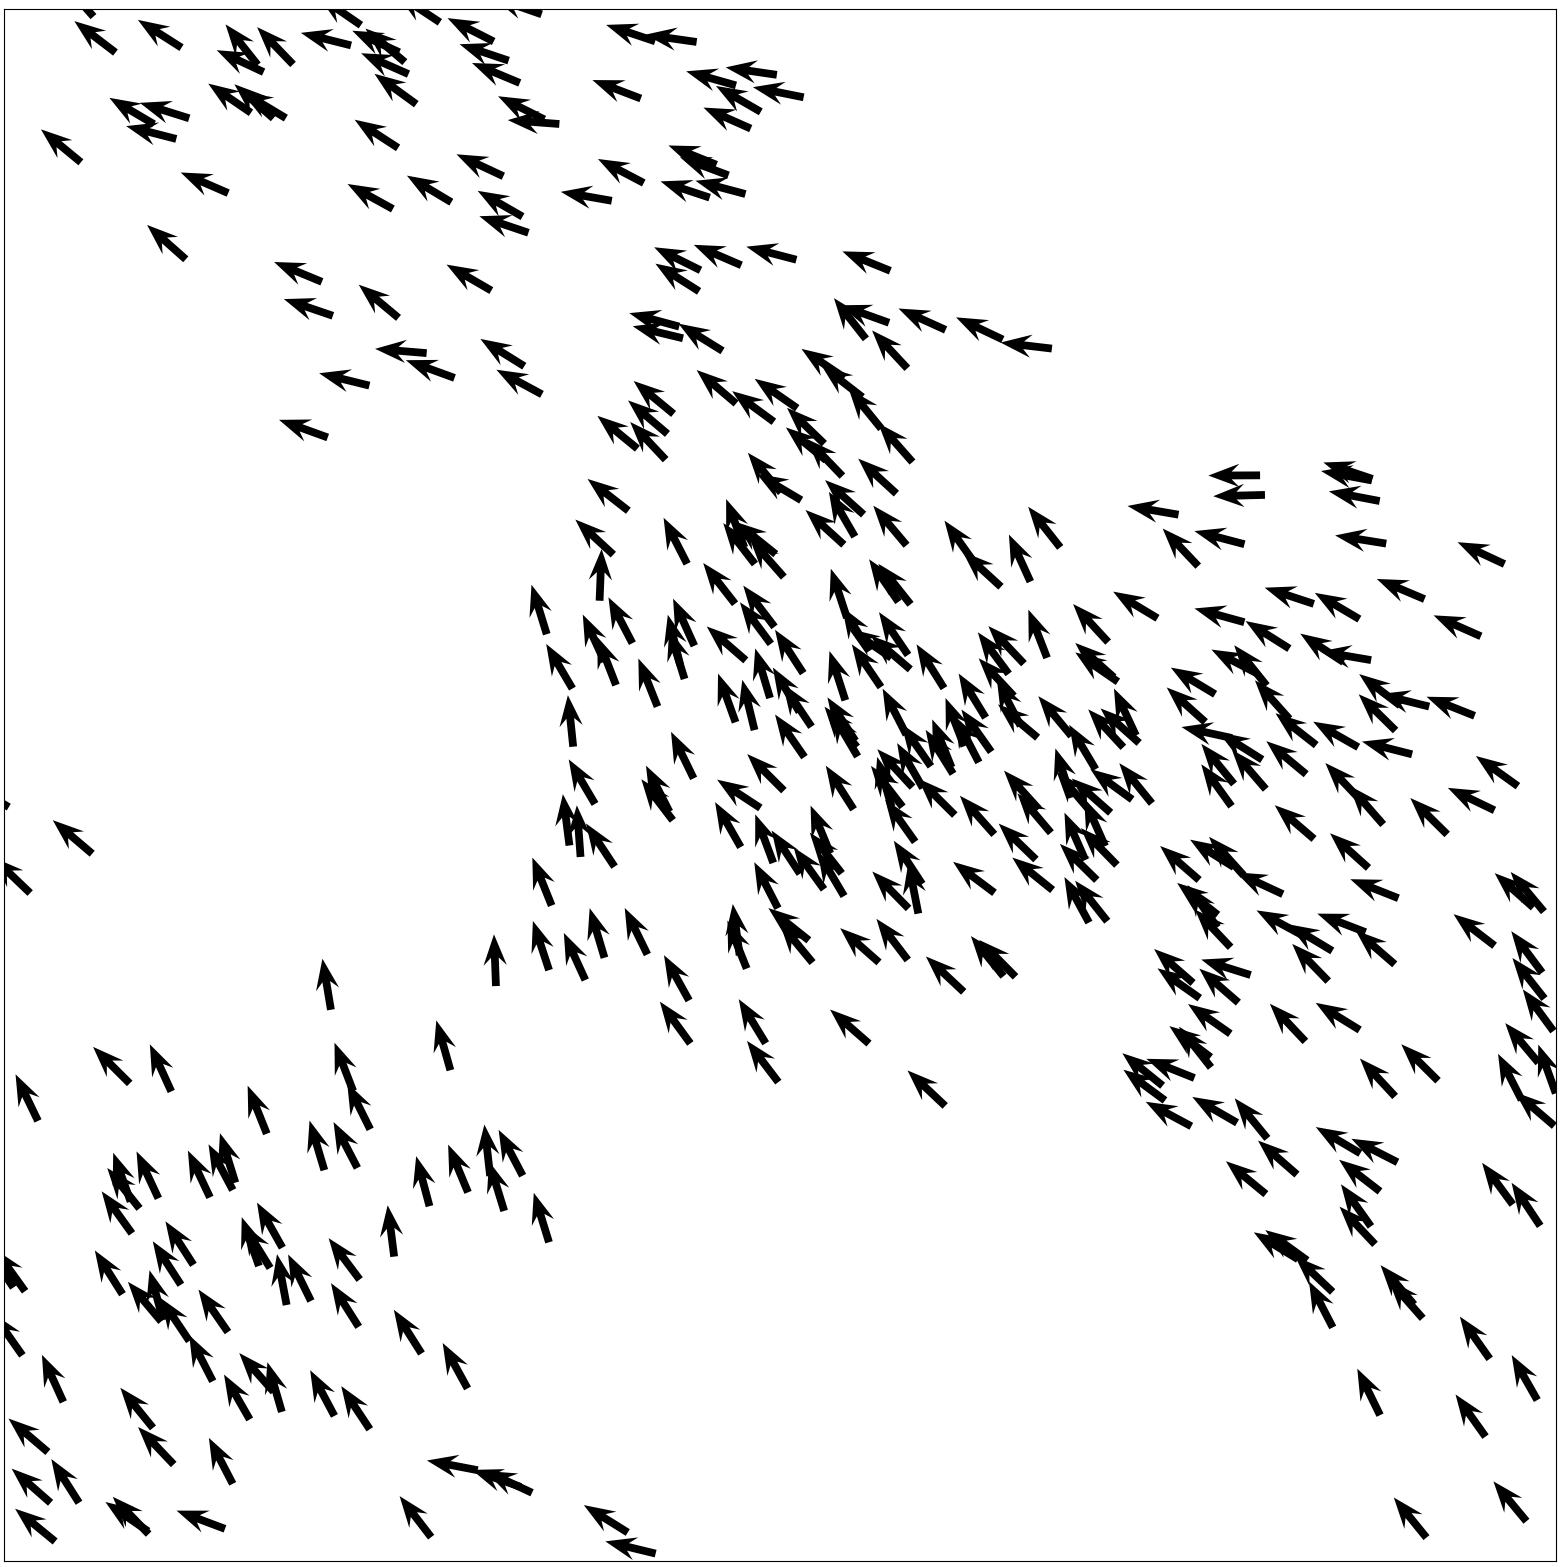
\includegraphics[width=0.28\textwidth]{figures/Snapshot_rk2_n0.6.png} &
    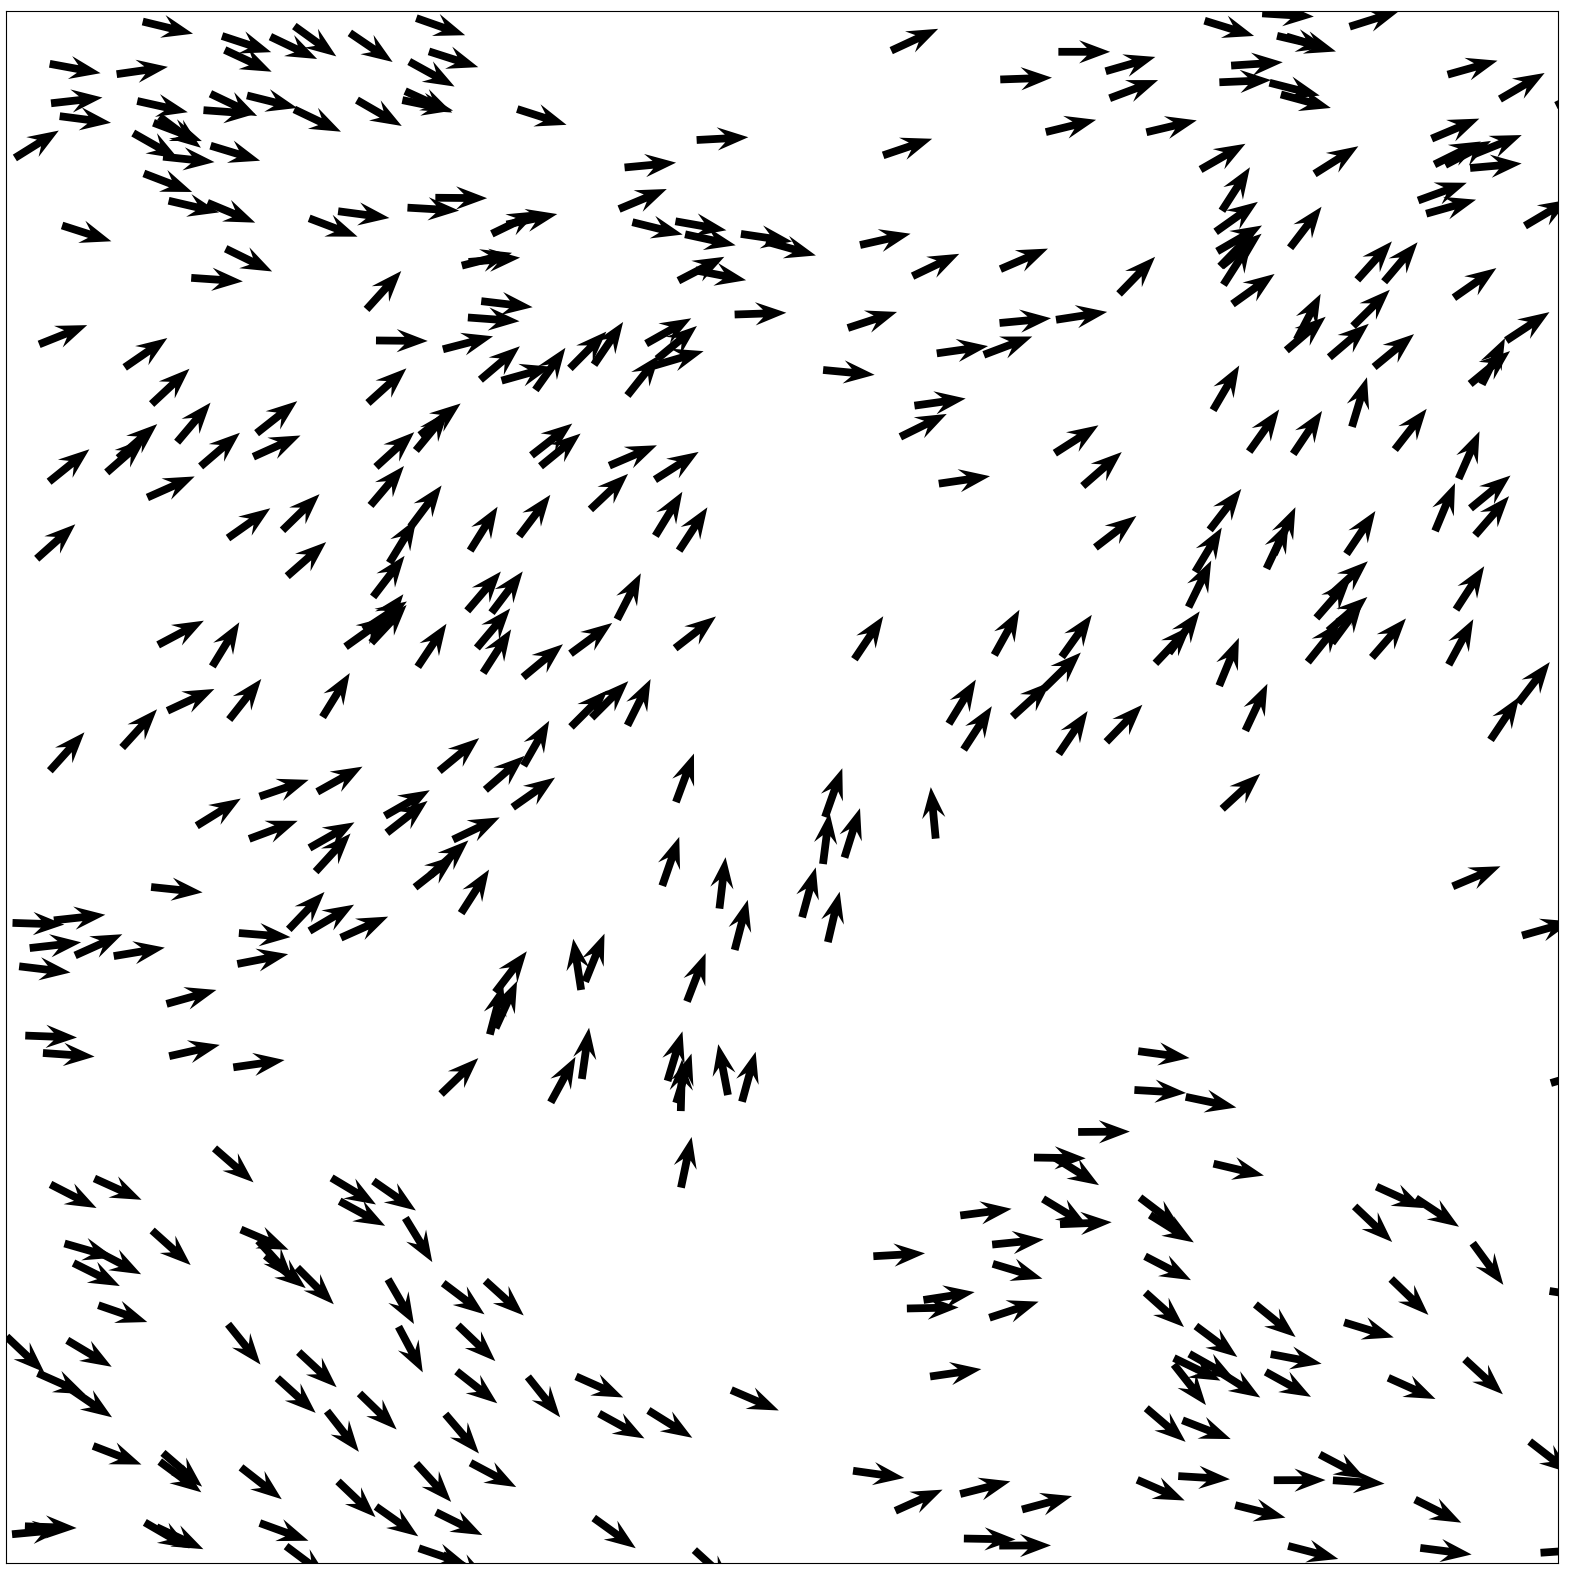
\includegraphics[width=0.28\textwidth]{figures/Snapshot_rk4_n1.0.png} \\
    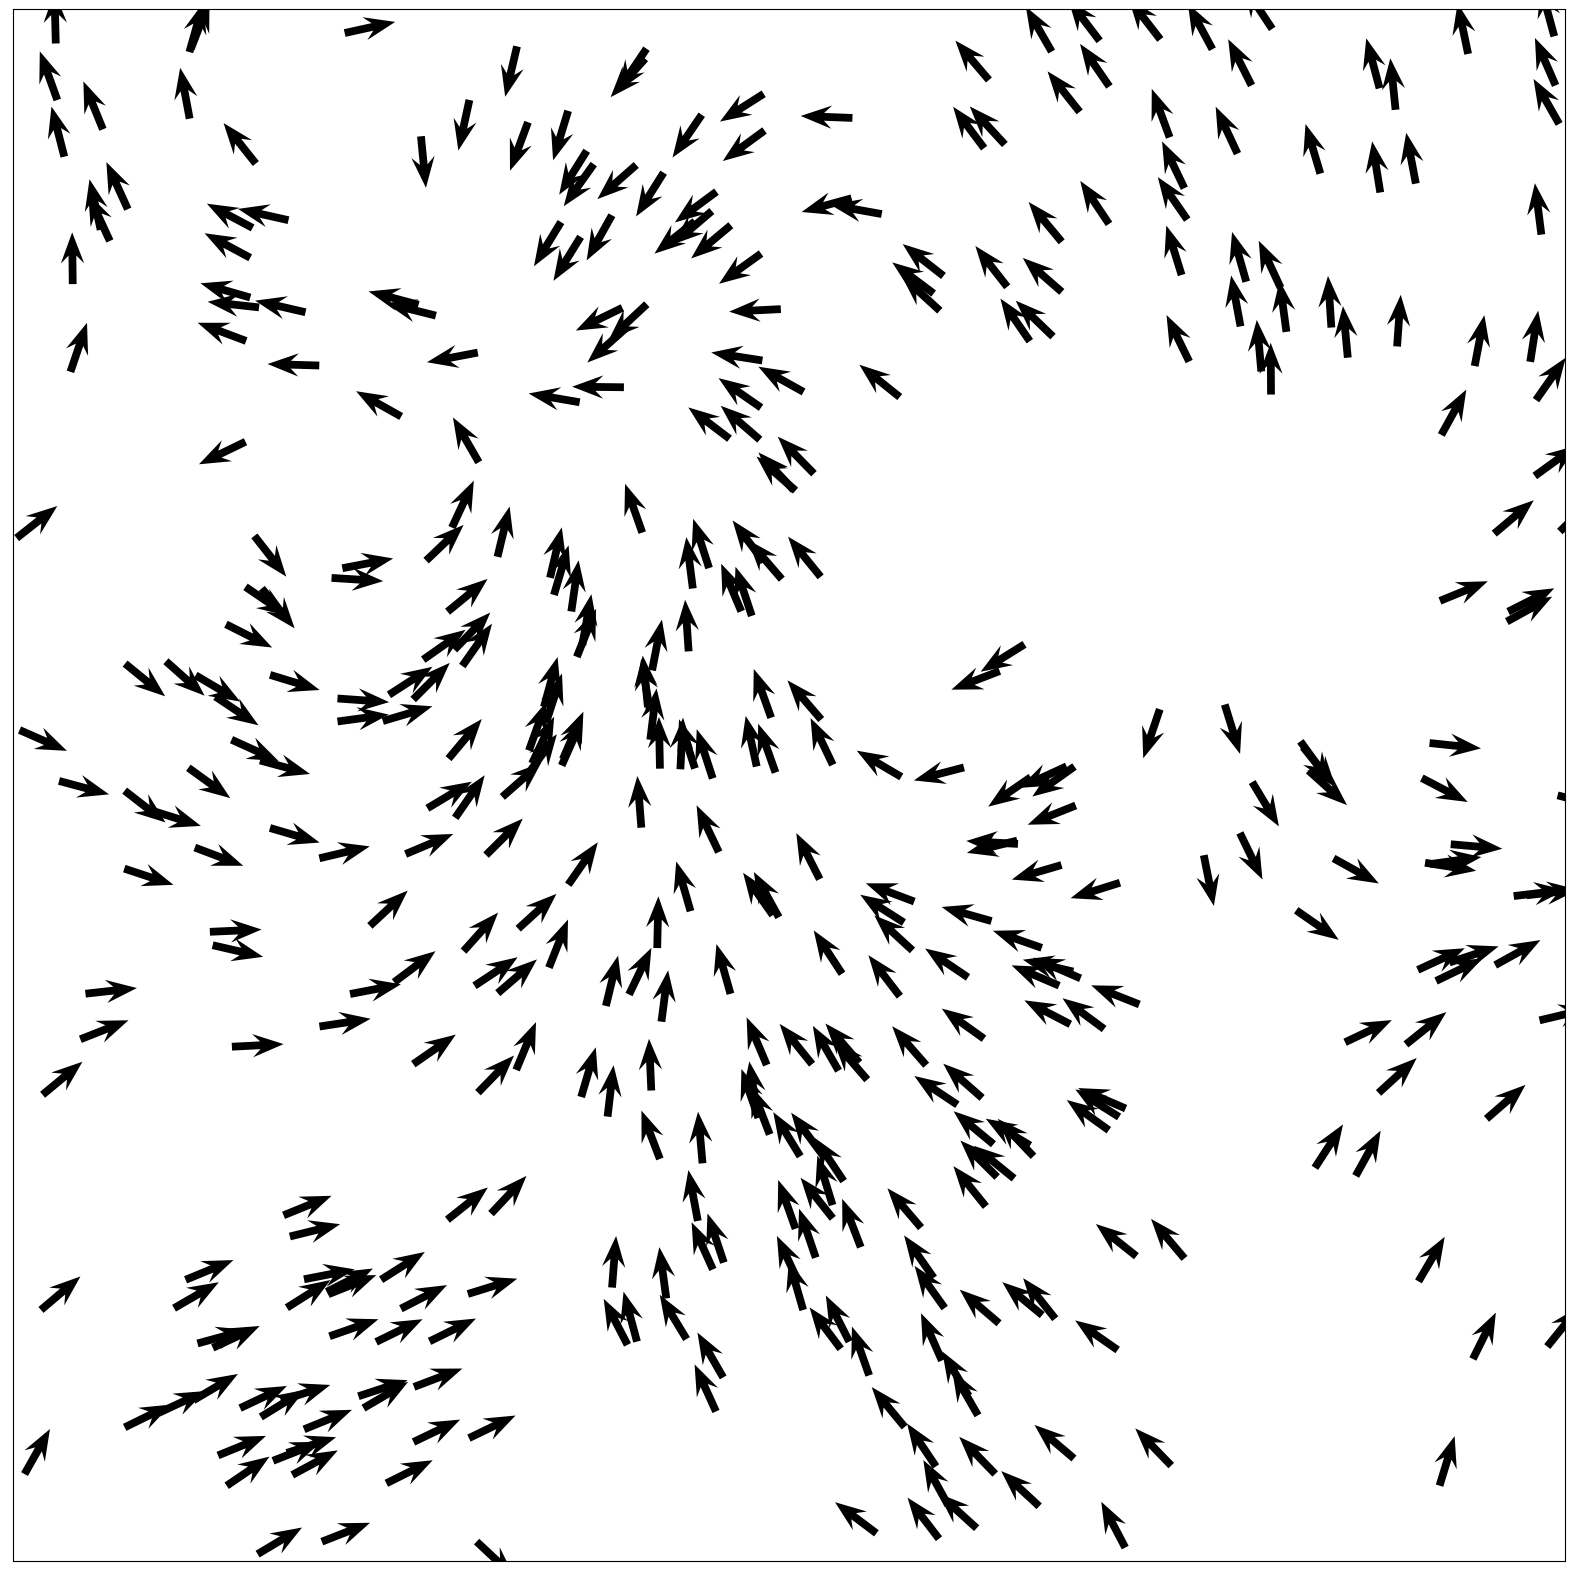
\includegraphics[width=0.28\textwidth]{figures/Snapshot_r1_n0.4.png} &
    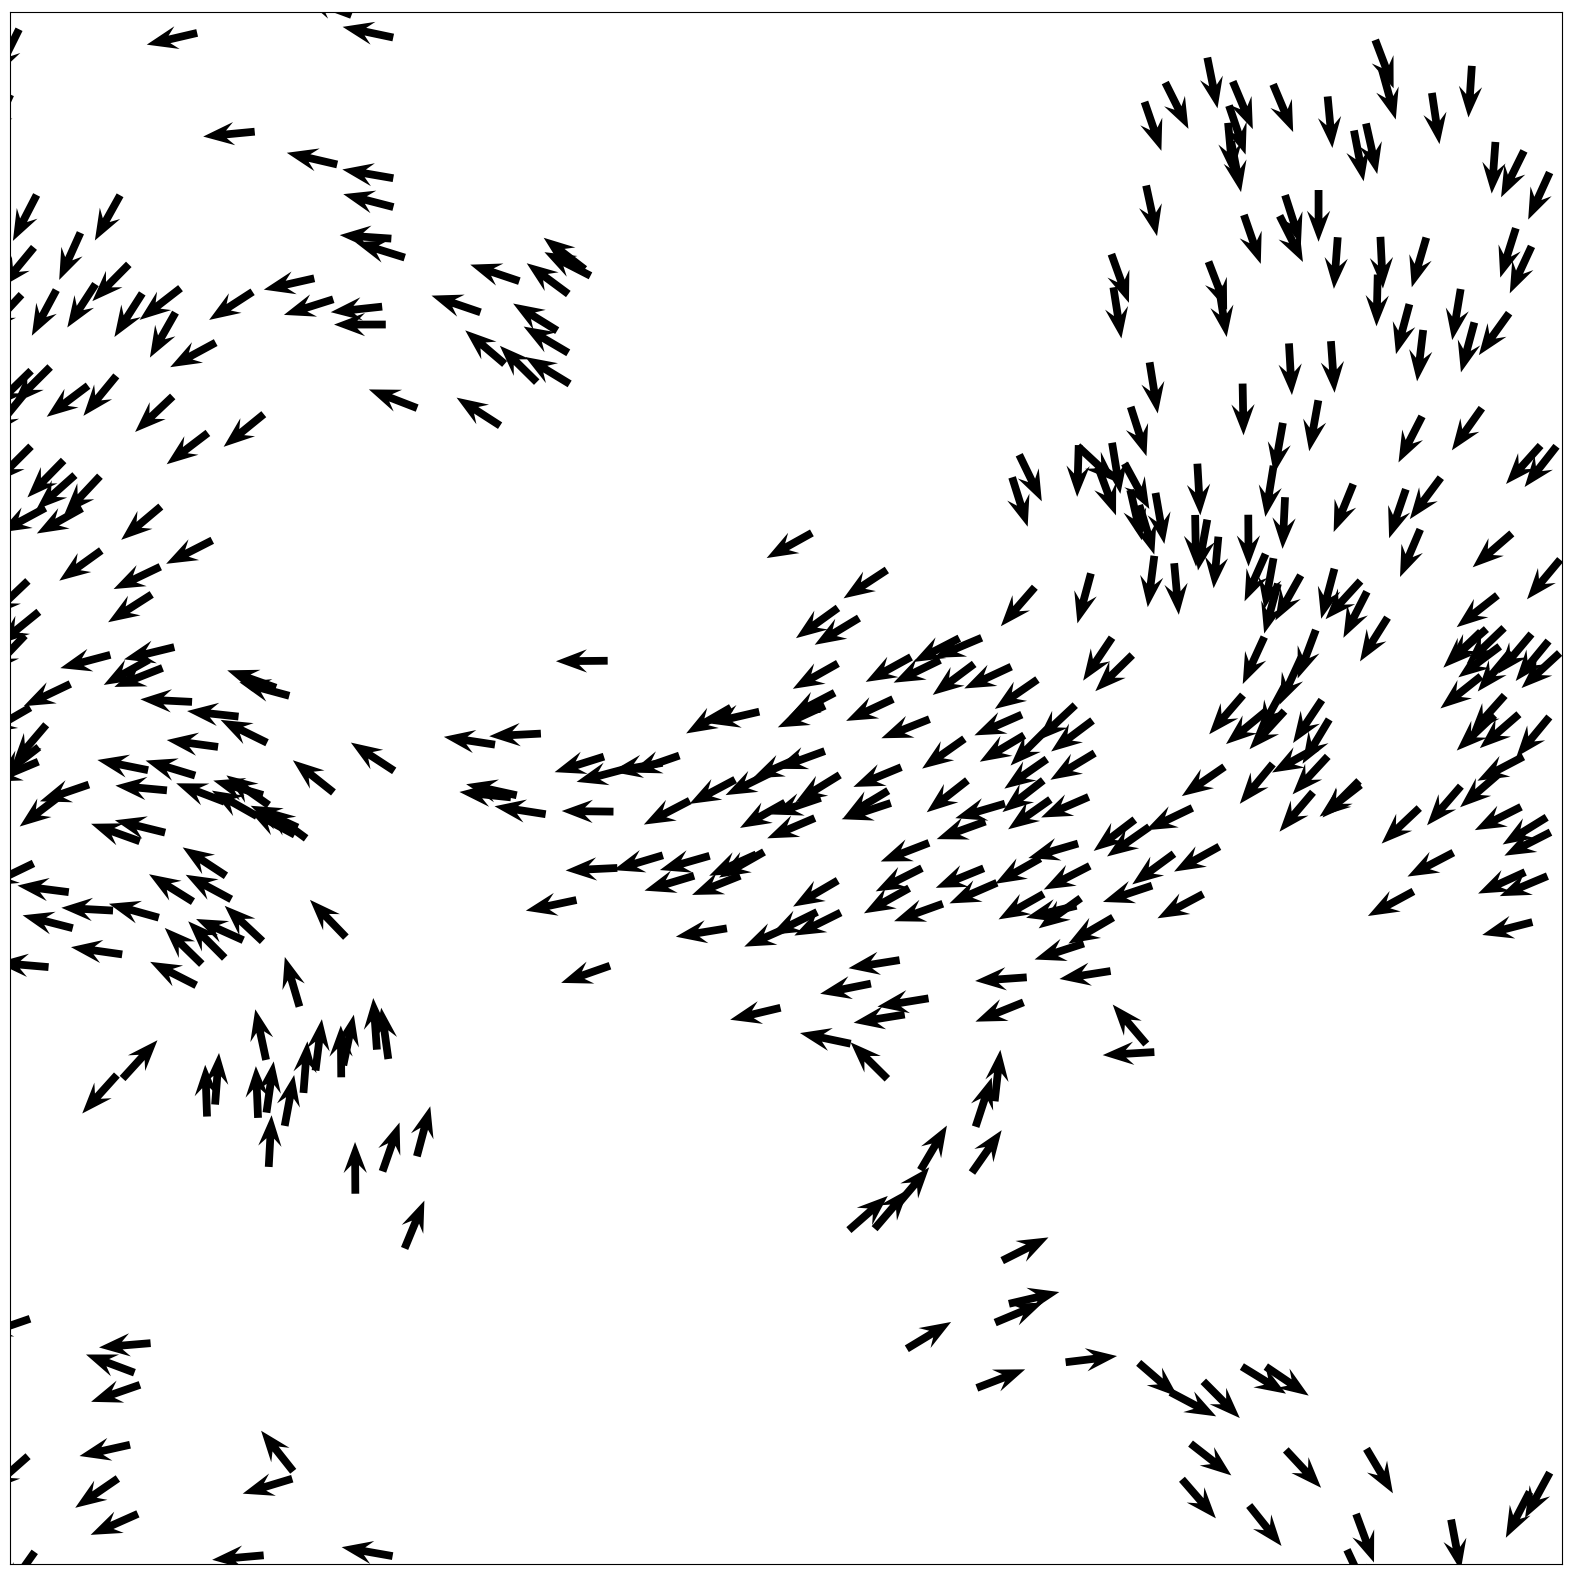
\includegraphics[width=0.28\textwidth]{figures/Snapshot_r1_n0.6.png} &
    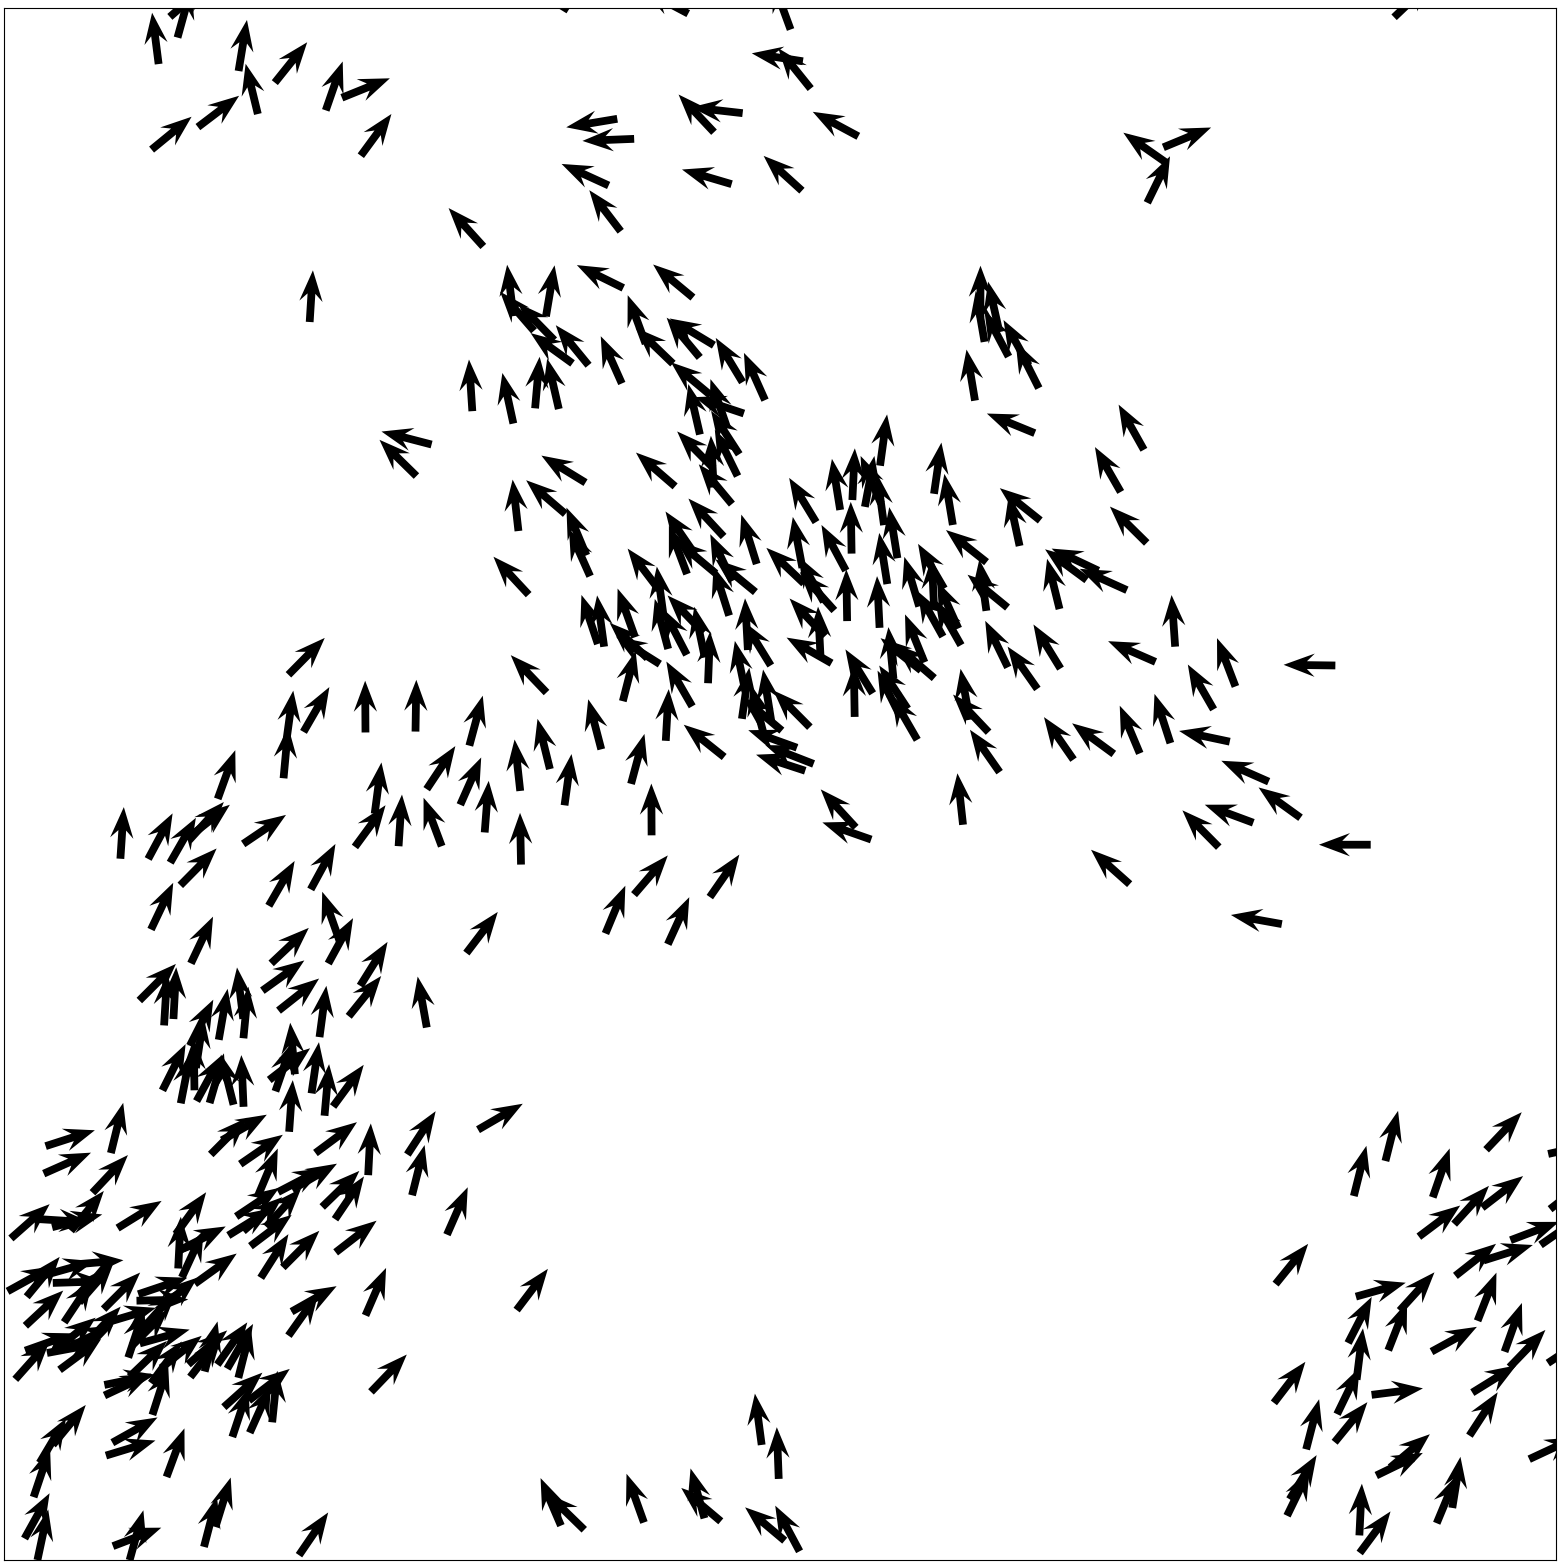
\includegraphics[width=0.28\textwidth]{figures/Snapshot_r1_n1.0.png}
    \end{tabular}
    \caption{Snapshots of the three models after few simulation steps,
    with $N=400$ and $\rho=4$. Columns from left to right:
    $\eta=0.4$ ($k=1$), $\eta=0.6$ ($k=2$), $\eta=1.0$ ($k=4$).
    Top row: purely topological model. The swarm fragments into many
    small aligned packets. Middle row: the stochastic
    metric-topological model introduced in this thesis. Although only
    $k$ neighbors are used per step, large stream-like structures
    form. Bottom row: metric Vicsek reference. The middle row
    resembles the bottom row far more than the top row does.}
    \label{fig:snapshots}
\end{figure*}

Fixing the number of interaction partners is attractive: it makes the
input size of each agent constant, which matters both for biological
plausibility and for machine learning, where network inputs have a
fixed dimension. In practice, however, the purely topological Vicsek
variant behaves poorly in the investigated regimes. In regions of
high local density the $k$ nearest neighbors are all very close, so
interactions become effectively short-ranged. Small packets of
mutually aligned agents form, decouple from the rest, and the global
order parameter collapses already at very small noise (top row of
Figure~\ref{fig:snapshots}; see also Figure~\ref{fig:topo_curves}).

\begin{figure*}[tb]
    \centering
    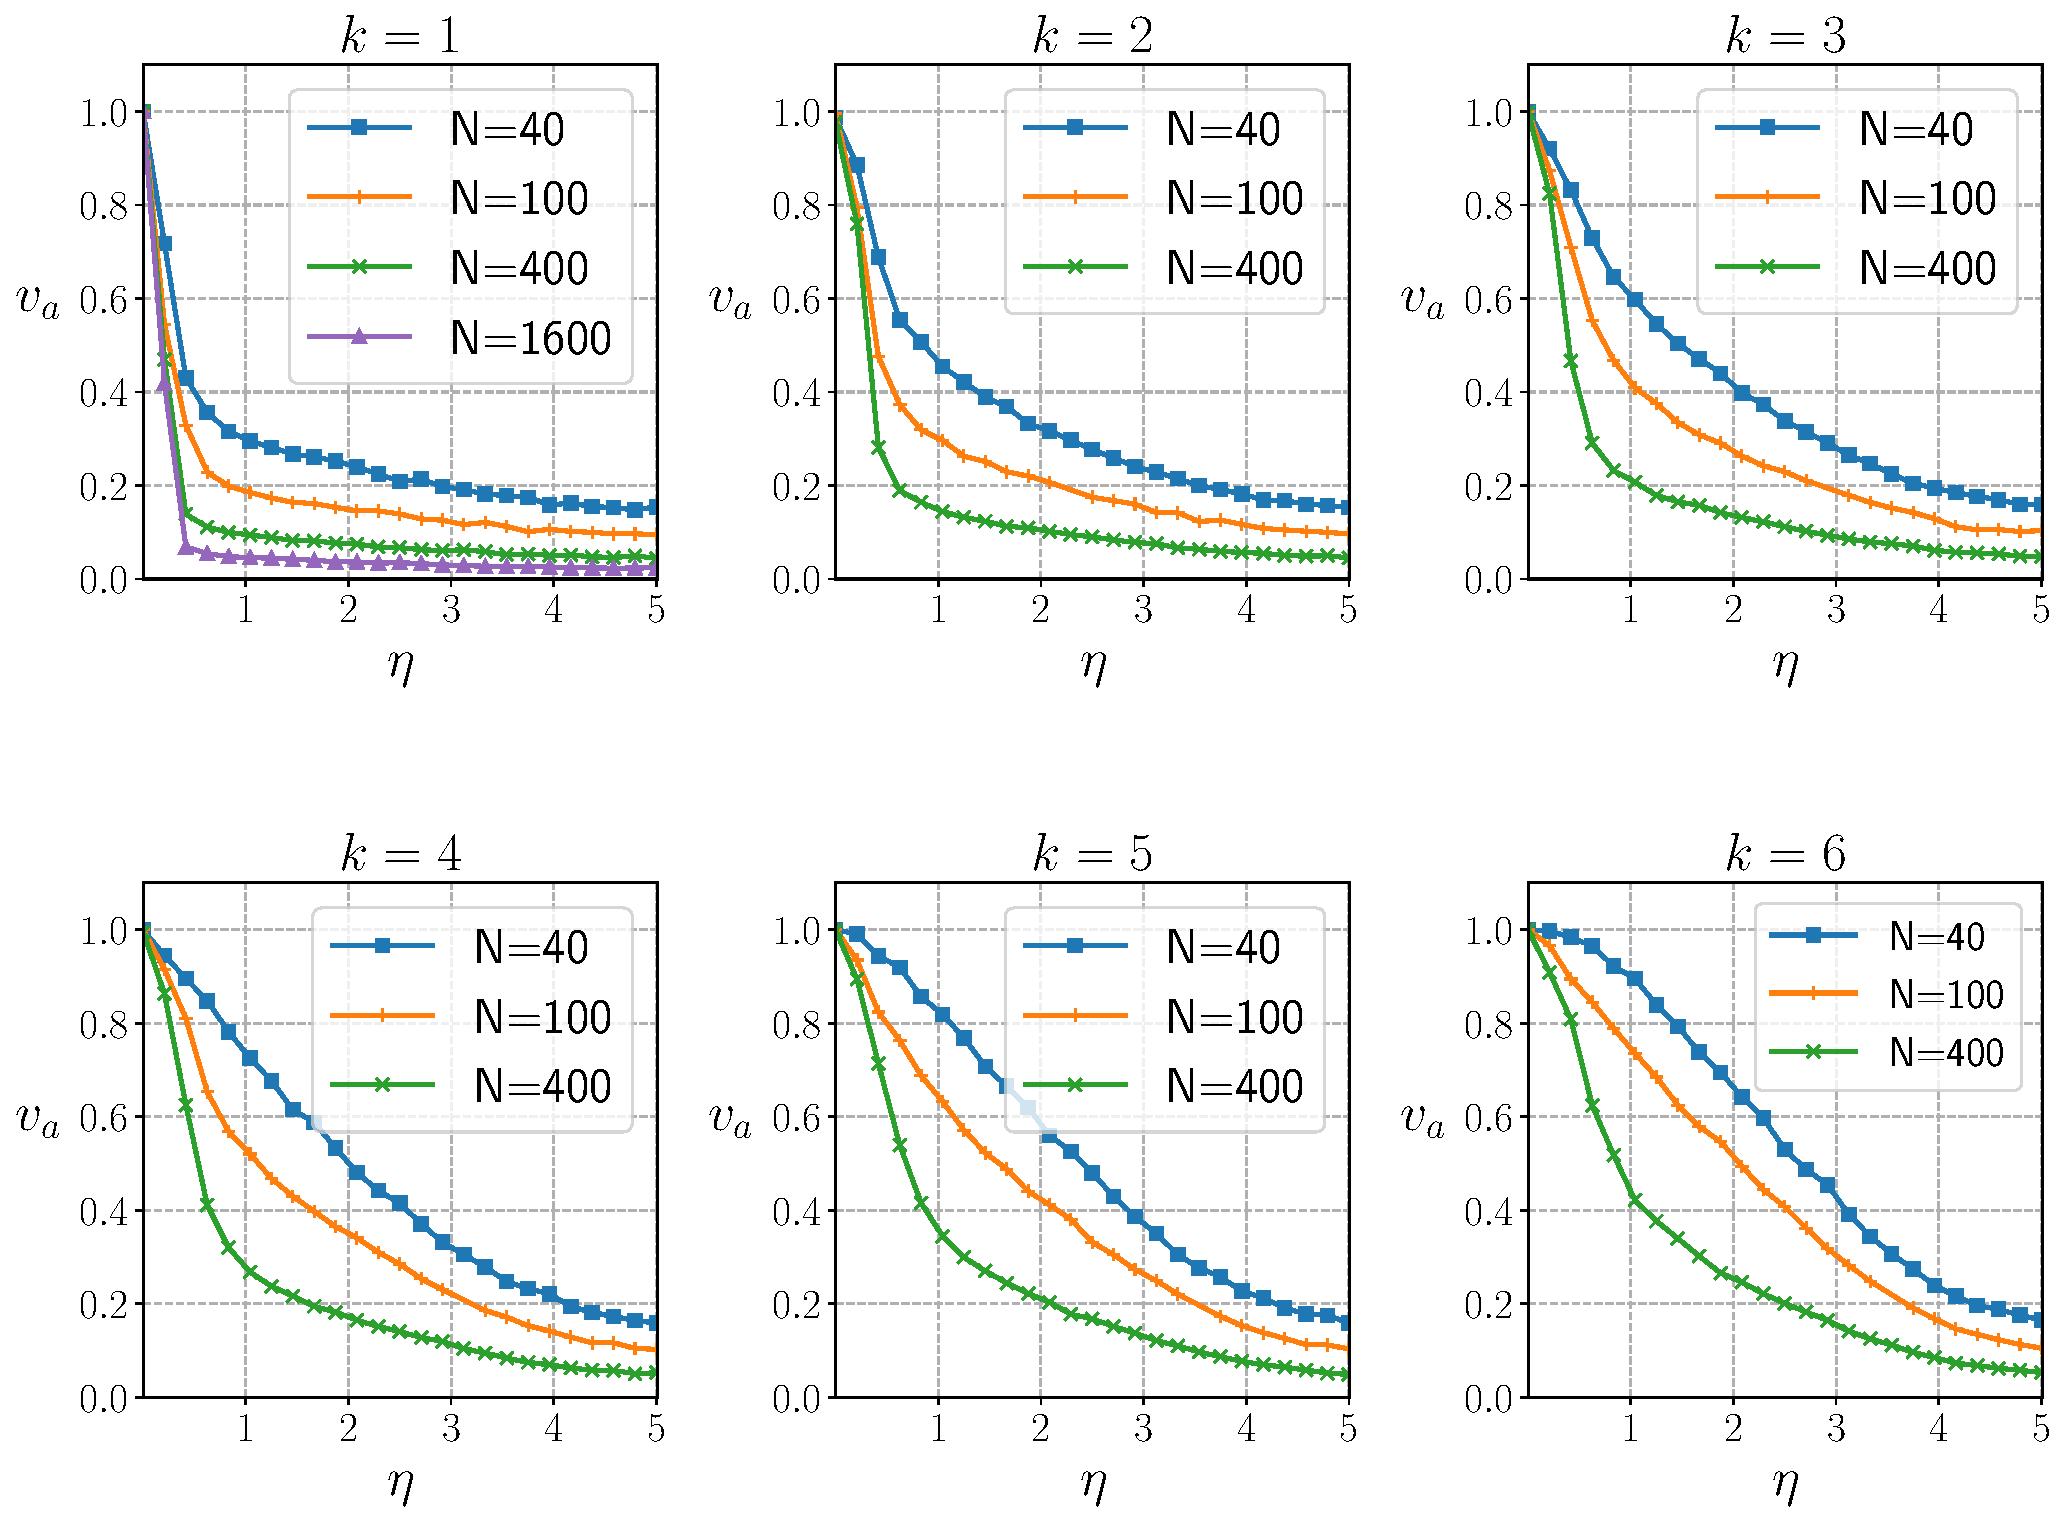
\includegraphics[width=0.92\textwidth]{figures/Vicsek_1a_kNeighbors_final.pdf}
    \caption{Order parameter $v_a$ versus noise $\eta$ for the purely
    topological model at constant density $\rho=4$, for
    $k=1$ to $6$ neighbors and several system sizes. For small $k$
    the order parameter collapses already at very small noise values,
    and larger systems are affected more strongly. This instability
    motivates the metric-topological rule.}
    \label{fig:topo_curves}
\end{figure*}

A naive repair, taking the $k$ nearest neighbors and discarding all
of them beyond the radius $r$, makes things worse: it removes exactly
the long-ranged part of the interaction that was still present.

\section{The stochastic metric-topological rule}

\begin{figure*}[tb]
    \centering
    
\includegraphics[width=0.42\textwidth]{figures/RadialHistogram_plain.pdf}
    \hspace{0.04\textwidth}
    
\includegraphics[width=0.42\textwidth]{figures/RadialHistogram_quantile.pdf}
    \caption{Conceptual motivation, shown for synthetic data. Left: a
    radial histogram of the headings an agent sees inside its
    interaction radius. Two larger groups with different orientations
    are visible. Right: the same histogram divided into $k$-quantiles
    (here $k=8$, dashed lines), regions that contain equal numbers of
    agents. Averaging one representative per region compresses the
    full neighborhood into $k$ inputs without discarding any
    direction of the sky. The random sampling rule realizes this
    averaging over time.}
    \label{fig:radial}
\end{figure*}

The model introduced in this thesis keeps both structural elements:
the metric radius $r$ and the fixed neighbor count $k$. The rule is:

\begin{enumerate}
    \setlength\itemsep{0pt}
    \item Collect all agents within the metric radius $r$
    (the Vicsek candidate set).
    \item If this set holds more than $k$ agents, draw $k$ of them
    uniformly at random, without replacement. Otherwise keep all.
    \item Apply the Vicsek average, Eq.~\eqref{eq:rule}, to the
    sampled set (plus the agent itself).
\end{enumerate}

The draw is repeated independently for every agent and every time
step, so the interaction graph is resampled continuously.

\paragraph{Intuition.}
Figure~\ref{fig:radial} shows the idea that led to the rule. Seen
from one agent, the neighborhood is a radial histogram of headings.
If the agent can only process $k$ inputs, a sensible compression is
to divide the histogram into $k$ regions of equal agent count
($k$-quantiles) and average within each region. Computing quantiles
explicitly every step is expensive. Random sampling achieves the same
effect statistically: over many steps, uniform draws hit each
equal-count region equally often.

\paragraph{Monte Carlo interpretation.}
The quantities that enter the Vicsek average are the sample means of
$\sin\theta$ and $\cos\theta$ over the selected neighbors. Under
uniform sampling without replacement, these sample means are unbiased
estimators of the means over the full metric neighborhood. Each
update is therefore a Monte Carlo estimate of the exact Vicsek
update, with $k$ in the role of the sample size. This view makes a
clear prediction: the model should converge to the metric Vicsek
model as $k$ grows. Section~\ref{sec:results} confirms this
empirically. No variance or error control was implemented; the
estimate is simply plugged into the dynamics at small fixed $k$.

\section{Simulation and validation}

\begin{figure*}[tb]
    \centering
    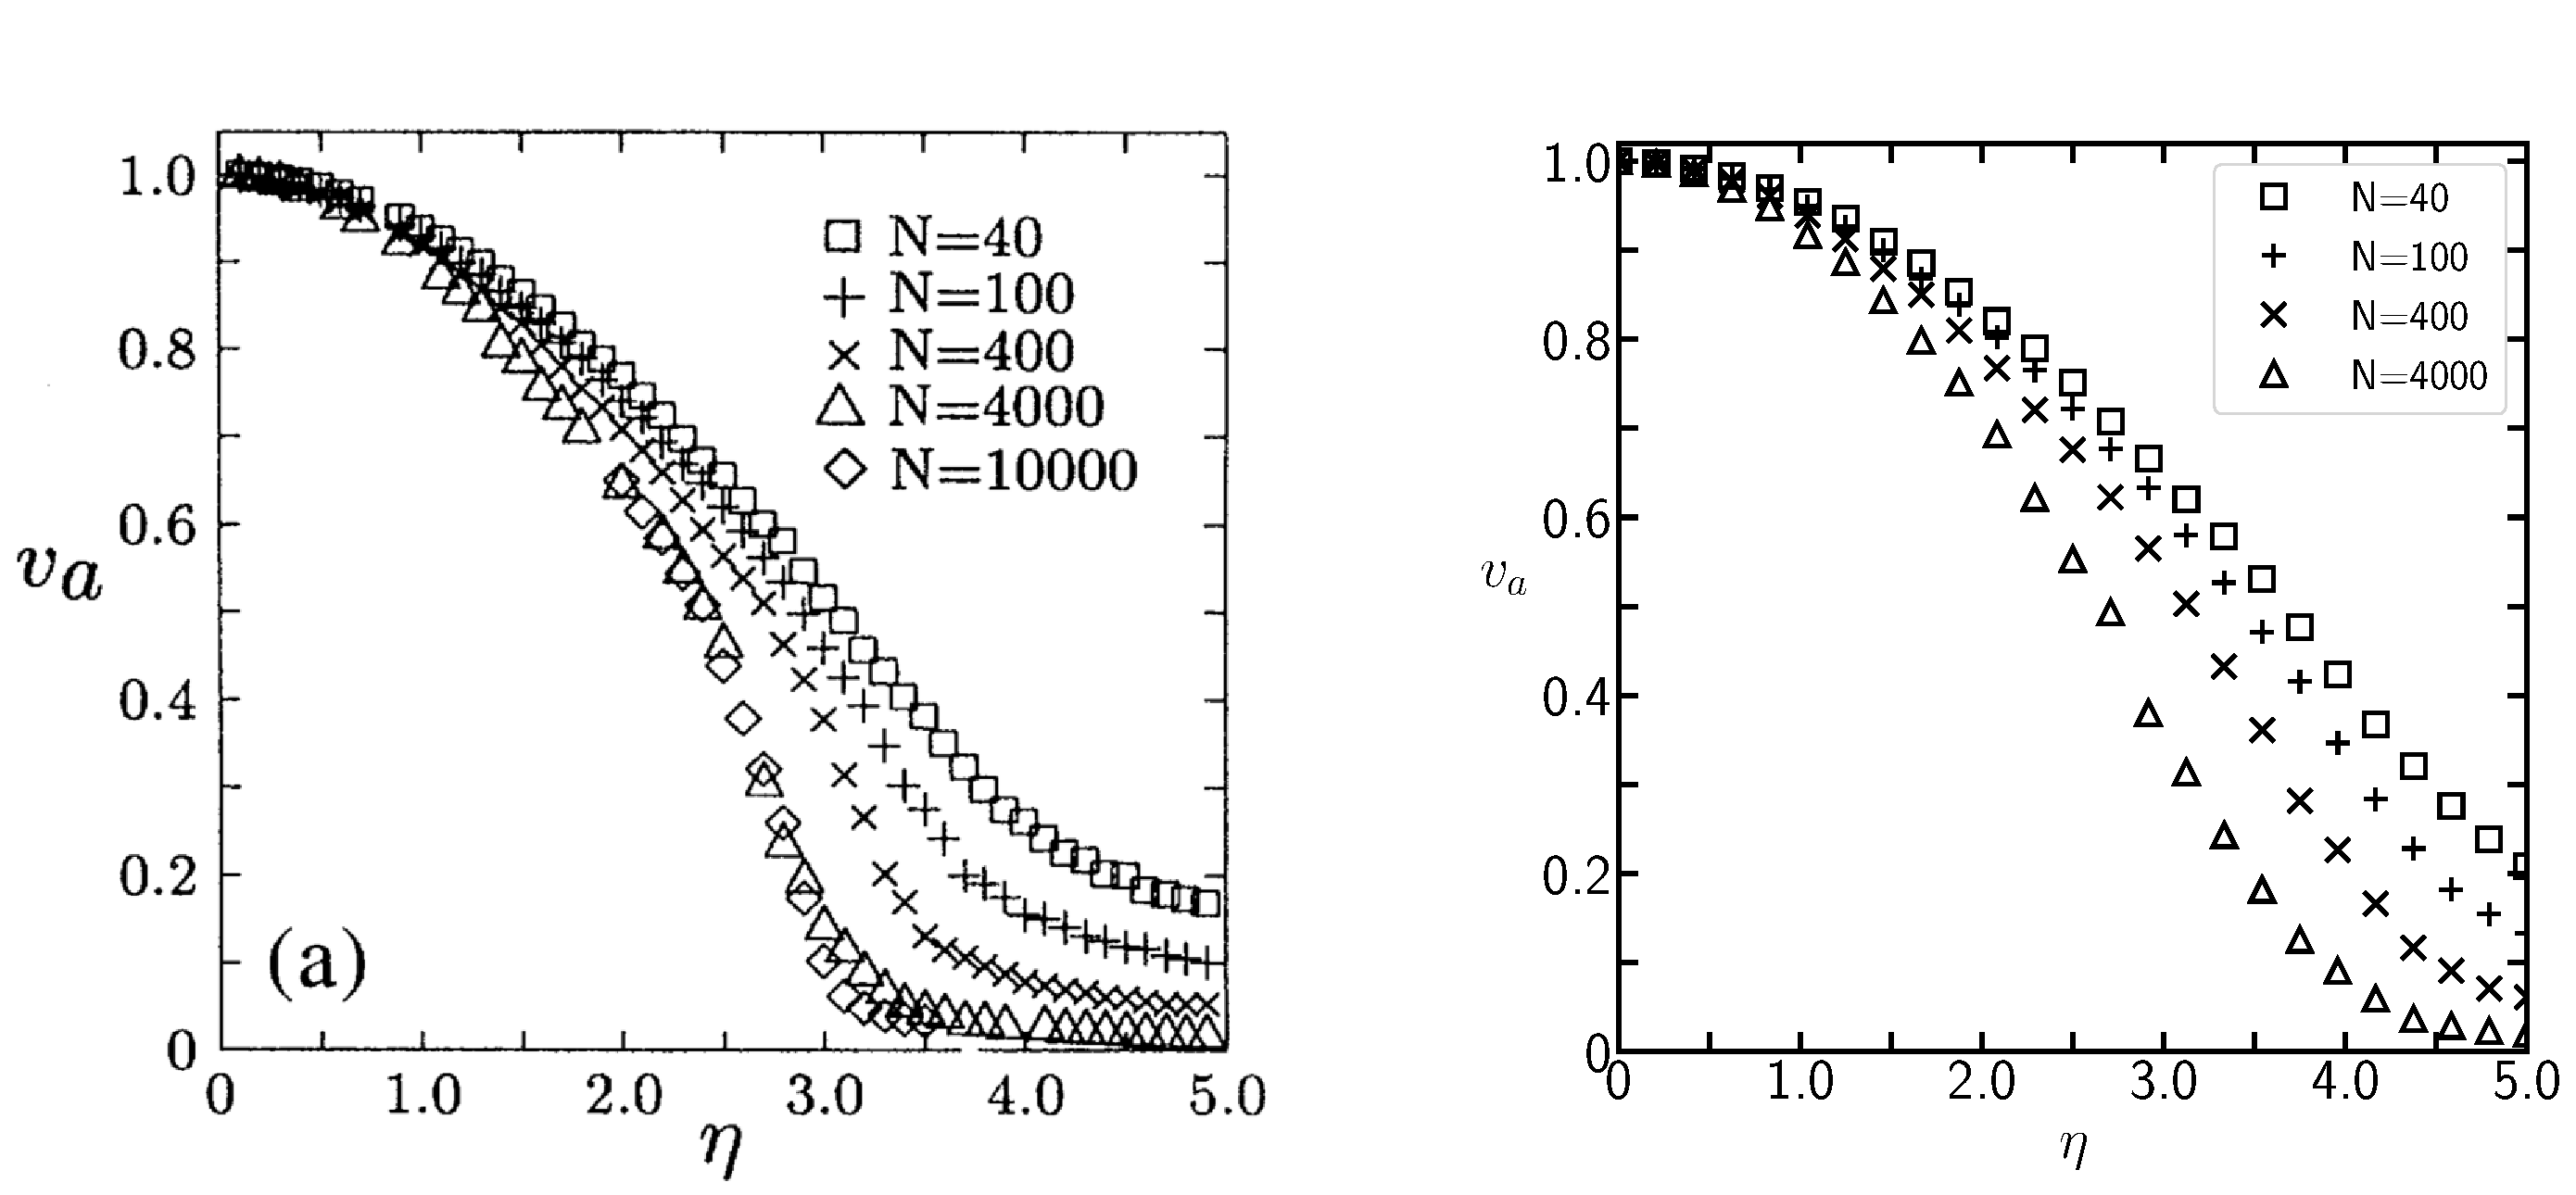
\includegraphics[width=0.88\textwidth]{figures/Vicsek_1a_rRadius_final.pdf}
    \caption{Validation of the simulation core. Left: the original
    measurement from Vicsek et al.\ \cite{vicsek1995}, order
    parameter $v_a$ versus noise $\eta$ at constant density. Right:
    the same experiment reproduced with the simulation written for
    this thesis. The qualitative course agrees; deviations appear for
    large noise ($\eta \gtrsim 3$) and are discussed in the thesis.}
    \label{fig:validation}
\end{figure*}

The simulation core is written in C++ \cite{cpp14} and exposed to
Python \cite{python310} through pybind11 \cite{pybind11}. C++ handles
the performance-critical parts, Python handles orchestration,
analysis, and plotting with Matplotlib \cite{Matplotlib2007}. The
core solves four recurring tasks:

\begin{itemize}
    \setlength\itemsep{0pt}
    \item \textbf{Cell decomposition.} The box is divided into square
    cells of edge length $2r$ and agents are assigned to cells. The
    neighbor search then only inspects a small cell neighborhood
    instead of all $\mathcal{O}(N^2)$ pairs.
    \item \textbf{Neighbor determination.} All model variants share
    one neighbor routine; the metric, topological, and
    metric-topological rules differ only in the final selection step.
    This step dominates the runtime and is the only part that is
    parallelized with OpenMP.
    \item \textbf{Periodic boundaries.} Distances and cell lookups
    are corrected for wrap-around, which has to be respected at
    several layers of the code.
    \item \textbf{Synchronous updates.} All agents are updated from
    the same previous state, as in the original model.
\end{itemize}

Large runs are written as \texttt{.xyz} trajectories and rendered
with OVITO \cite{OVITO2010}, a visualization tool from solid state
physics that handles up to $10^5$ agents in real time. In addition,
an interactive Matplotlib front end with live sliders for $\eta$,
$r$, and $k$, an optional cell grid overlay, and per-neighbor
distance lines was built for visual debugging. This visual
inspection layer proved essential for catching boundary and neighbor
selection errors that unit checks missed.

Before any comparison between models, the metric baseline itself was
validated against the original publication.
Figure~\ref{fig:validation} reproduces the classic order parameter
versus noise measurement of Vicsek et al.\ \cite{vicsek1995}. The
curves agree qualitatively over the full noise range; quantitative
deviations at high noise ($\eta \gtrsim 3$) remain and several
candidate error sources (neighbor search, boundary handling, random
number generators, statistical protocol) were checked and excluded in
the thesis. Stability of the measured values was checked by varying
simulation length and initial conditions, including fully ordered
starts; results converged to the same values.

\section{Results}
\label{sec:results}

\begin{figure*}[tb]
    \centering
    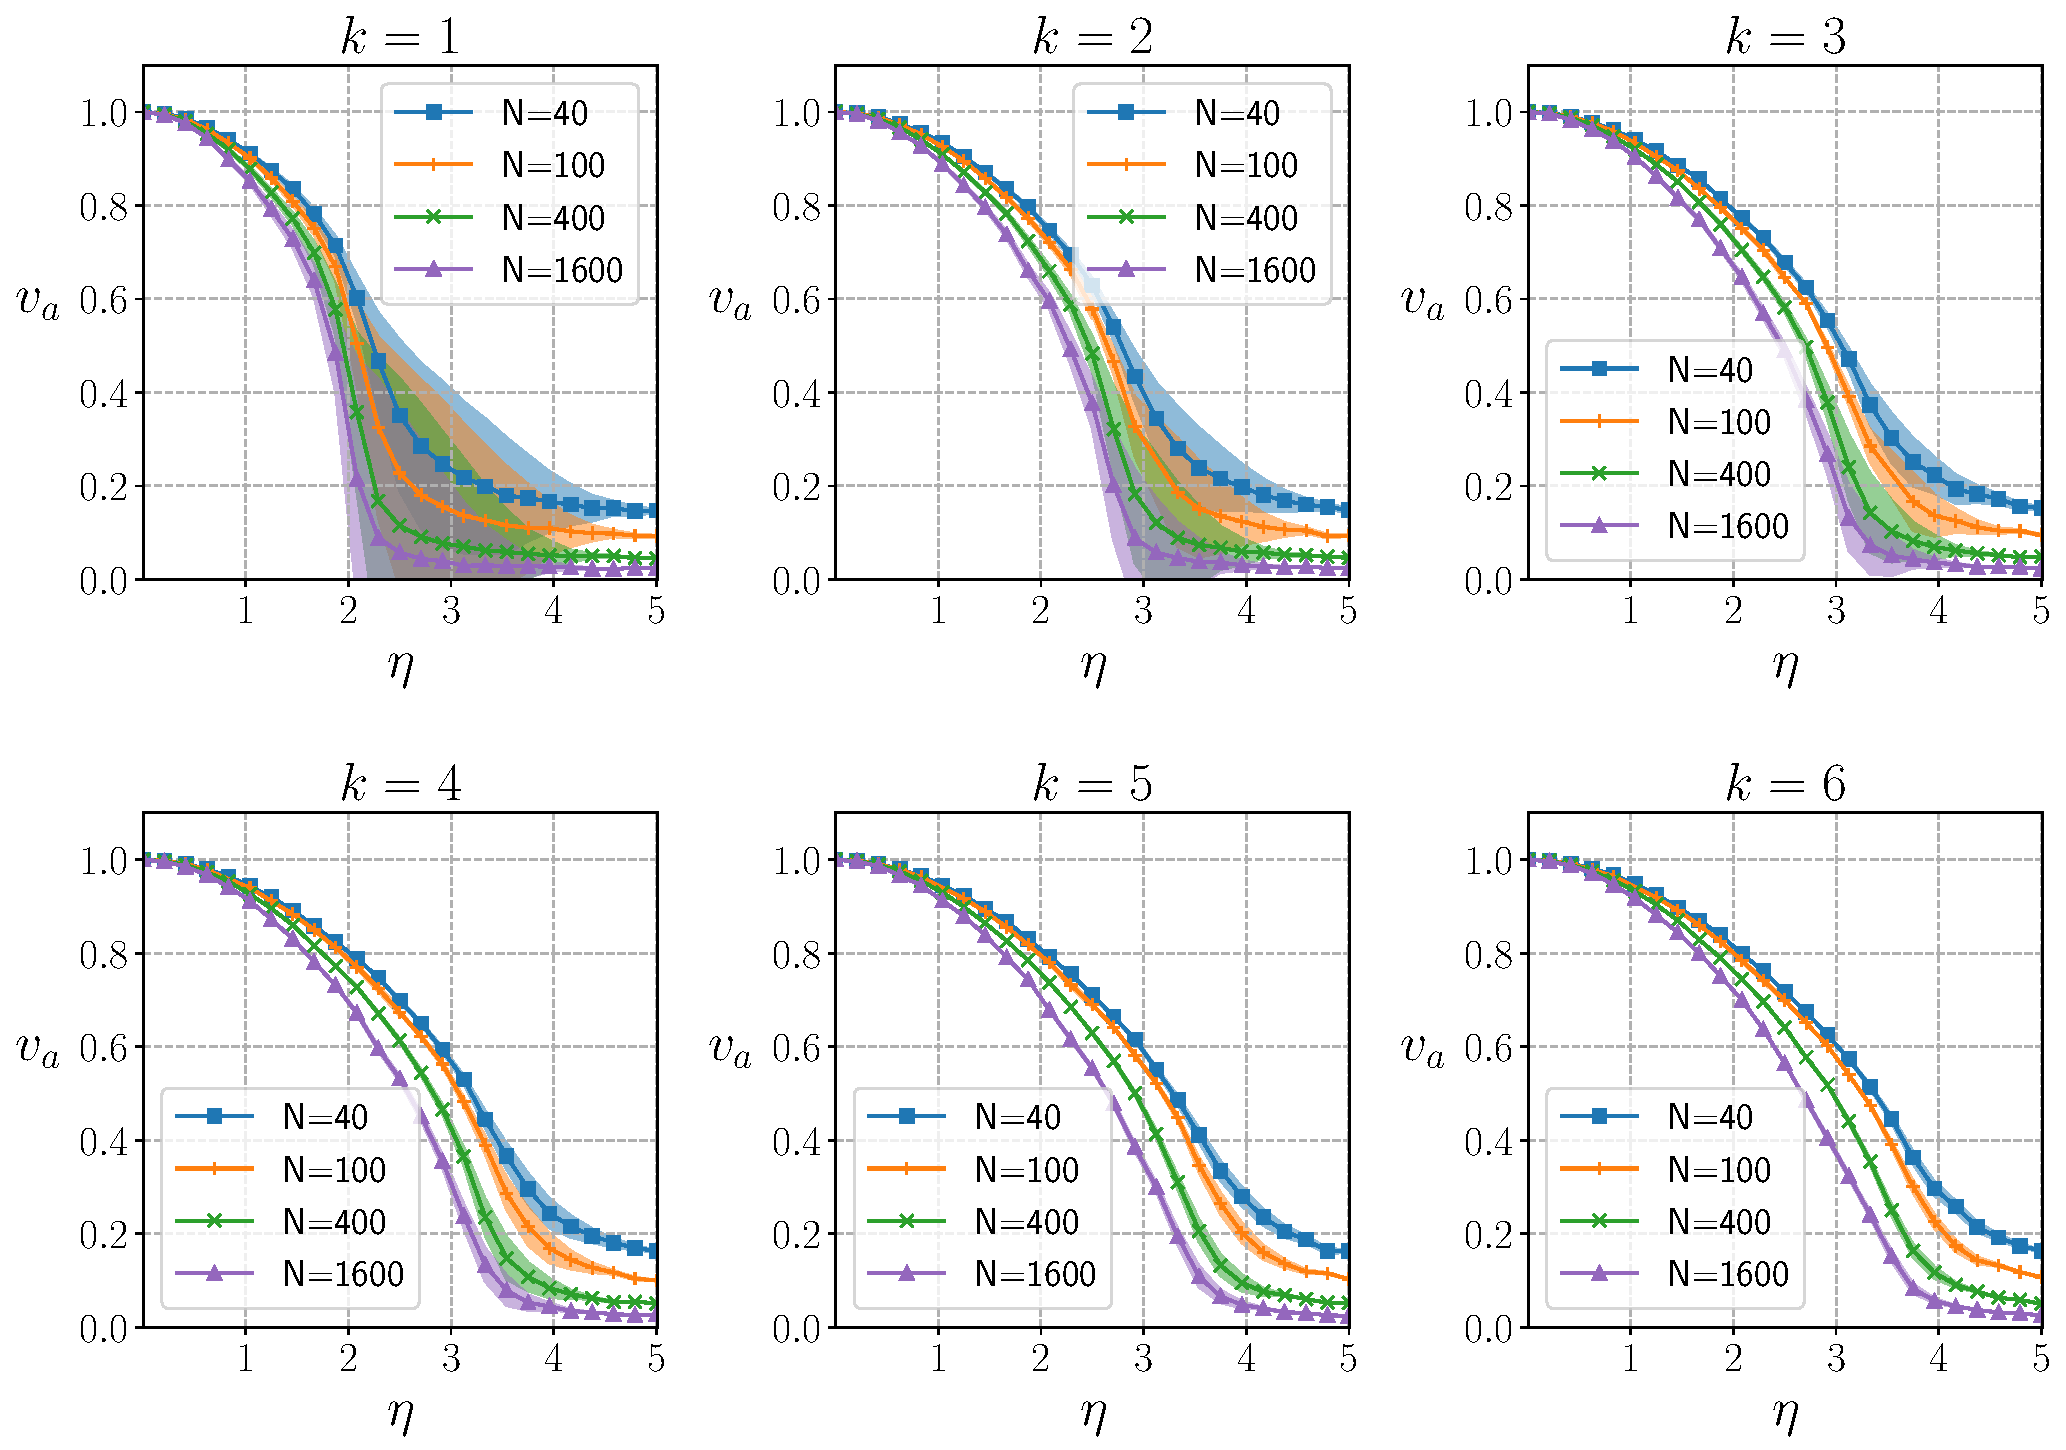
\includegraphics[width=\textwidth]{figures/Convergence_1a_rkFixedRadius_final.pdf}
    \caption{Convergence of the stochastic metric-topological model
    toward the metric Vicsek model at constant density $\rho=4$.
    Each panel shows $v_a(\eta)$ for one value of $k$ and several
    system sizes; the shaded tube around each curve is the squared
    deviation from the Vicsek reference. The tubes shrink quickly
    with growing $k$; for $k=6$ the deviations are barely visible.}
    \label{fig:convergence}
\end{figure*}

\begin{figure*}[tb]
    \centering
    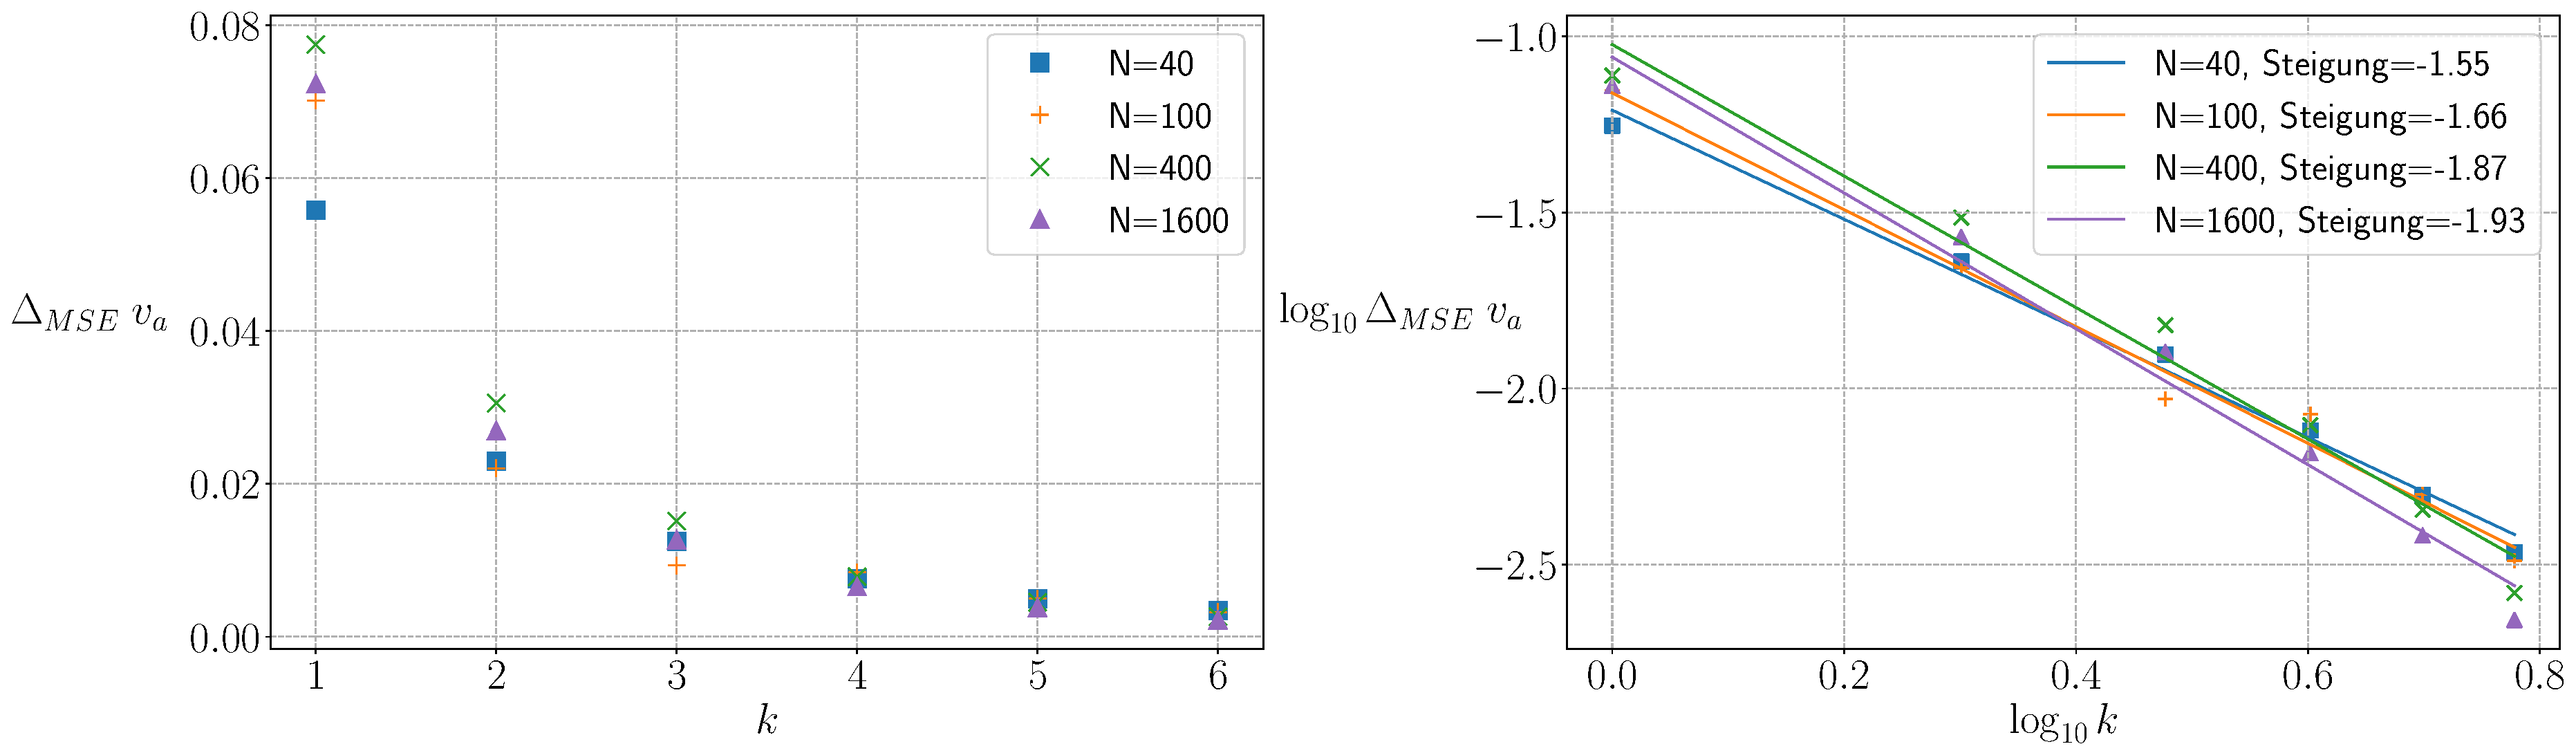
\includegraphics[width=0.92\textwidth]{figures/MSE_vs_k_double.pdf}
    \caption{Quantitative convergence in the sample size $k$. Left:
    mean squared deviation of $v_a$ between the metric-topological
    model and the self-generated Vicsek reference, for each system
    size and $k = 1$ to $6$. Right: log-log representation with
    linear fits (the German legend word ``Steigung'' means slope).
    The deviation follows an approximate power law in $k$ with fitted
    slopes between $-1.55$ and $-1.93$; larger systems converge more
    slowly at equal density.}
    \label{fig:mse}
\end{figure*}

\paragraph{Stability.}
The middle row of Figure~\ref{fig:snapshots} shows the qualitative
result. Although each agent uses only $k$ neighbors per step, the
fragmentation of the purely topological model disappears. The swarm
forms large stream-like structures that resemble the metric Vicsek
reference. One visible difference remains: sharp vortex-like turns of
the metric model are smoothed out for small $k$, because an agent
cannot process all incoming directions in a single step.

\paragraph{Convergence to the Vicsek model.}
For $k \geq N$ the rule keeps every candidate and reduces exactly to
the metric Vicsek model, so convergence in $k$ is expected. The
Monte Carlo interpretation predicts that it should be fast.
Figure~\ref{fig:convergence} shows $v_a(\eta)$ for $k=1$ to $6$ with
the squared deviation from the Vicsek reference drawn as a tube
around each curve. Figure~\ref{fig:mse} condenses this into a single
number per configuration: the mean squared deviation falls by more
than an order of magnitude from $k=1$ to $k=6$, approximately as a
power law in $k$, and for $k=6$ the two models are practically
indistinguishable under this observable. Larger systems converge
more slowly at equal density.

These statements are limited to the evaluated observable
($v_a$ as a function of $\eta$), the evaluated densities, and system
sizes up to $N=1600$ for the quantitative comparison. No claim of
general equivalence is made.

\paragraph{Density-based order parameter.}
The alignment parameter $v_a$ says nothing about how compact a swarm
is: a system of many small, internally aligned packets and one large
coherent flock can score identically. To close this gap, the thesis
additionally introduced a distance-weighted order parameter,
\begin{equation}
    \rho_a \propto
    \sum_{i<j}^{N} \tilde{\vec{v}}_i \cdot \tilde{\vec{v}}_j
    \left( \left|\tilde{\vec{x}}_i - \tilde{\vec{x}}_j\right|^2
    + d^2 \right)^{-\alpha/2},
    \label{eq:densityop}
\end{equation}
where the smoothing scale $d$ caps the contribution of very close
pairs and $\alpha$ controls how strongly distance is weighted. Pairs
that are aligned and close contribute most, so $\rho_a$ rewards
compact coherent swarms. It was implemented and measured for the
metric-topological model, but only studied phenomenologically. Such
parameters are also natural candidates for reward signals in the
learning experiments of the next section, because they encode a
global goal in a single scalar.

\section{Reinforcement learning extension}

\begin{figure}[tb]
    \centering
    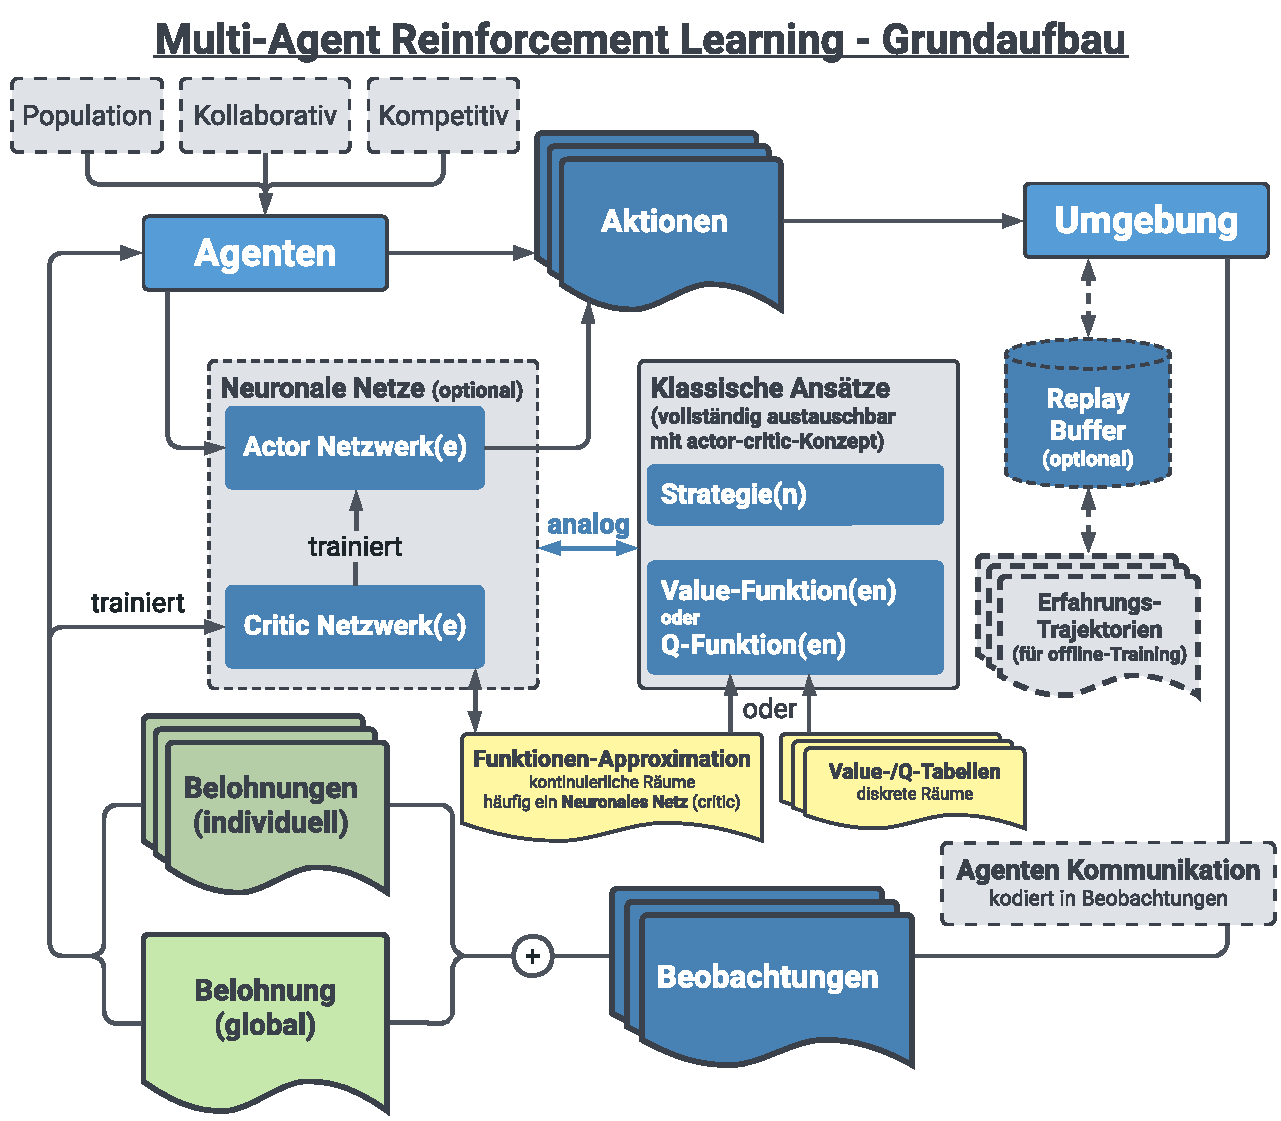
\includegraphics[width=\linewidth]{figures/MARL_Grundaufbau.pdf}
    \caption{Conceptual MARL setup drawn for the thesis: agents act
    in a shared environment, observations and rewards flow back, and
    an actor network selects actions while a critic network estimates
    their value. Labels are in German (``Agenten'' agents,
    ``Aktionen'' actions, ``Umgebung'' environment, ``Belohnungen''
    rewards, ``Beobachtungen'' observations).}
    \label{fig:marl}
\end{figure}

\begin{figure}[tb]
    \centering
    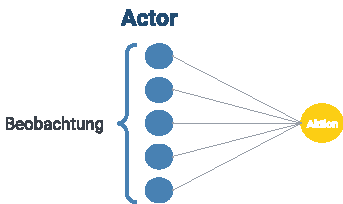
\includegraphics[width=0.8\linewidth]{figures/Actor_Netzwerk.pdf}
    \caption{The actor network used in the experiments
    (``Beobachtung'' means observation, ``Aktion'' means action). It
    was kept deliberately minimal (a single dense layer) because the
    target behavior, the Vicsek averaging rule, is itself a simple
    function of the observed neighbor headings.}
    \label{fig:actor}
\end{figure}

The second goal of the thesis was a change of perspective: instead of
prescribing a local interaction rule, define a global objective and
let the agents learn the rule. The order parameter
Eq.~\eqref{eq:orderparam} is a natural reward signal, since the
Vicsek rule itself drives $v_a$ upward. The metric-topological model
was designed with this in mind, because its fixed $k$ gives every
agent an observation vector of constant size.

\paragraph{Setup.}
Figure~\ref{fig:marl} shows the conceptual architecture. The C++
simulation was wrapped as a learning environment through pybind11: a
dedicated simulation class hands each agent the headings of its $k$
sampled neighbors as the observation, accepts a new heading in
$[0, 2\pi]$ as the continuous action, and reports the change of the
global order parameter as the reward. On this environment an
actor-critic pipeline \cite{DDPG, TFAgents, tensorflow2015-whitepaper}
was trained, with the minimal actor of Figure~\ref{fig:actor} and a
standard critic. A second attempt used a multi-agent environment with
one agent per particle and a shared policy in RLlib \cite{RLlib}.

\paragraph{Outcome.}
The pipeline ran end to end: environment, replay buffer, actor,
critic, and training loop all worked together, and training
proceeded. The results, however, were not interpretable. The main
identified problem was the representation of the angle: a heading is
a periodic quantity, and feeding it to the networks as a plain scalar
in $[0, 2\pi]$ creates a discontinuity at the wrap-around that the
simple networks did not overcome in the available time. The RLlib
attempt failed earlier, at training launch. No successful or
partially successful policy was obtained, and no conclusion about the
learnability of the Vicsek rule can be drawn from these experiments.
What the thesis does establish is that the simulation is fully
embeddable in standard MARL tooling, and it formulates the natural
next experiment: testing whether a single-layer perceptron with a
periodic angle encoding (for example $\sin\theta$, $\cos\theta$) can
learn the averaging rule.

\section{Limitations and outlook}

The scope of the positive result is deliberately narrow. Agreement
with the Vicsek model was shown for the alignment order parameter
$v_a$ under the evaluated noise values, densities, and system sizes.
Other observables, such as correlation functions or the
density-based order parameter, were only touched on. The statistical
protocol used running averages without advanced error analysis, and
the high-noise deviation from the original Vicsek data remains
unexplained. The reinforcement learning part is a documented negative
result and should be read as such.

Natural continuations are: a periodic encoding of the heading for the
learning experiments; a variance analysis of the sampling rule to
put the Monte Carlo view on quantitative footing; and a study of the
model in regimes where metric and topological models genuinely
disagree, to see which behavior the mixed rule follows.

\medskip

The lasting value of the project is the combination of an original,
validated modeling idea with an early, honest attempt to connect
physical simulation and multi-agent learning.

\clearpage
\printbibliography

\end{document}
